\documentclass[11pt]{article}

\usepackage[margin=1in]{geometry}
\usepackage{amsmath,amsthm}
\usepackage{mathtools}
\usepackage{graphicx}
\usepackage{booktabs}
\usepackage{dsfont}  % \mathds{1} indicator
% Old-style journal look (matches ../../vdjtools/appendix): OldStandard text + matching OpenType
% math, small-caps headings, run-in paragraphs. Requires lualatex (pinned in .latexmkrc).
\usepackage{OldStandard}
\usepackage{unicode-math}
\setmathfont{OldStandard-Math.otf}
\usepackage{titlesec}
\usepackage{fancyvrb}
\usepackage[hidelinks]{hyperref}

\linespread{1.15}
\setlength{\parindent}{2em}
\titleformat{\section}{\normalfont\large\scshape\bfseries}{\thesection.}{0.6em}{}
\titleformat{\subsection}{\normalfont\scshape\bfseries}{\thesubsection.}{0.5em}{}
\titleformat{\paragraph}[runin]{\bfseries\scshape}{}{0pt}{}[.]
\titlespacing*{\paragraph}{\parindent}{0.4em}{0.6em}

\newtheoremstyle{oldplain}{}{}{\itshape}{}{\scshape}{.}{.5em}{}
\newtheoremstyle{oldrem}{}{}{\normalfont}{}{\scshape}{.}{.5em}{}
\theoremstyle{oldplain}
\newtheorem{proposition}{Proposition}
\newtheorem{lemma}{Lemma}
\theoremstyle{oldrem}
\newtheorem{definition}{Definition}
\newtheorem{remark}{Remark}

\newcommand{\Pgen}{P_{\mathrm{gen}}}
\newcommand{\R}{\mathds{R}}  % dsfont blackboard (OldStandard-Math lacks some \mathbb glyphs)
\newcommand{\E}{\mathds{E}}
\newcommand{\junc}{\mathrm{junc}}
\newcommand{\code}[1]{\texttt{#1}}
\DeclarePairedDelimiter{\norm}{\lVert}{\rVert}
\DeclareMathOperator{\Cov}{Cov}

\title{Prototype embeddings for immune receptors:\\
  geometry, statistics, and the {\normalfont\scshape TCREMP} coordinate system}
\author{Mikhail Shugay\textsuperscript{1,2,3}\thanks{Correspondence:
  \href{mailto:mikhail.shugay@gmail.com}{mikhail.shugay@gmail.com}}}
\date{%
  \small
  \textsuperscript{1}Institute of Translational Medicine, Russian National Medical State University, Moscow, Russia\\
  \textsuperscript{2}Department of Genomics of Adaptive Immunity, Shemyakin--Ovchinnikov Institute of Bioorganic Chemistry RAS, Moscow, Russia\\
  \textsuperscript{3}Institute of Molecular Biology NAS RA, Erevan, Armenia\\[6pt]
  \normalsize\textit{Appendix T --- {\normalfont\scshape TCREMP} embedding geometry}%
}

\renewcommand{\thesection}{T.\arabic{section}}

\begin{document}
\maketitle

\begin{abstract}
\noindent
{\scshape TCREMP} \cite{Kremlyakova2025} embeds an immune receptor as the vector of its alignment
distances to a fixed set of \emph{prototype} receptors sampled from the V(D)J recombination model
\cite{Murugan2012,Sethna2019}. This appendix gives the mathematics behind that construction. We first
develop the general theory of \emph{prototype} (landmark) embeddings of a metric space --- their
Lipschitz and isometry properties, the negative-type condition under which the alignment dissimilarity
is an honest squared Hilbert distance \cite{Schoenberg1938}, the energy functional that makes
embedding-space Euclidean distance track pairwise alignment distance, and a landmark sample-complexity
bound (\S\ref{sec:foundations}--\S\ref{sec:metric}). We then specialise to immune receptors: taking the
prototype measure to be the generation distribution $\Pgen$ turns each coordinate into a Monte-Carlo
sketch of a receptor's relationship to the generative repertoire, which explains why the choice of
prototype source scarcely matters and yields the observed Gamma / extreme-value distribution laws
(\S\ref{sec:immune}). The three-component structure of the {\scshape TCR} embedding and paired-chain
concatenation are read off as a product metric, with the germline blocks provably low-rank
(\S\ref{sec:tcr}); somatic hypermutation is a bounded perturbation that explains why {\scshape IGH} is
the hardest chain (\S\ref{sec:igh}); and the pushforward of $\Pgen$ onto embedding space is the null
model for density-based background subtraction (\S\ref{sec:density}). Every quantitative claim is
reproduced in-repo (\S\ref{sec:insights}, Table~\ref{tab:reproduced}) by \code{mir/bench/theory.py}.
\end{abstract}

\section{Foundations of prototype embeddings}\label{sec:foundations}

\paragraph{Setup} Let $(X,d)$ be a (semi)metric space of receptor sequences: $d$ is symmetric,
$d(x,x)=0$, and --- as we verify for the alignment dissimilarity in \S\ref{sec:metric} ---
non-negative. Fix an ordered set of \emph{prototypes} $P=\{p_1,\dots,p_K\}\subset X$. The
\textbf{prototype embedding} is the landmark map
\begin{equation}\label{eq:embedding}
  \varphi : X \to \R^{K}, \qquad \varphi(x) = \bigl(d(x,p_1),\,d(x,p_2),\,\dots,\,d(x,p_K)\bigr),
\end{equation}
and the induced \textbf{embedding distance} is $D(x,y)=\norm{\varphi(x)-\varphi(y)}_2$. Figure~\ref{fig:schematic}
shows the pipeline. In {\scshape TCREMP} the prototypes are drawn from $\Pgen$, $d$ is a BLOSUM alignment
dissimilarity, and $\varphi$ carries three coordinate blocks per prototype (\S\ref{sec:tcr}); the
foundational results below hold for any $(X,d,P)$.

\begin{figure}[t]
  \centering
  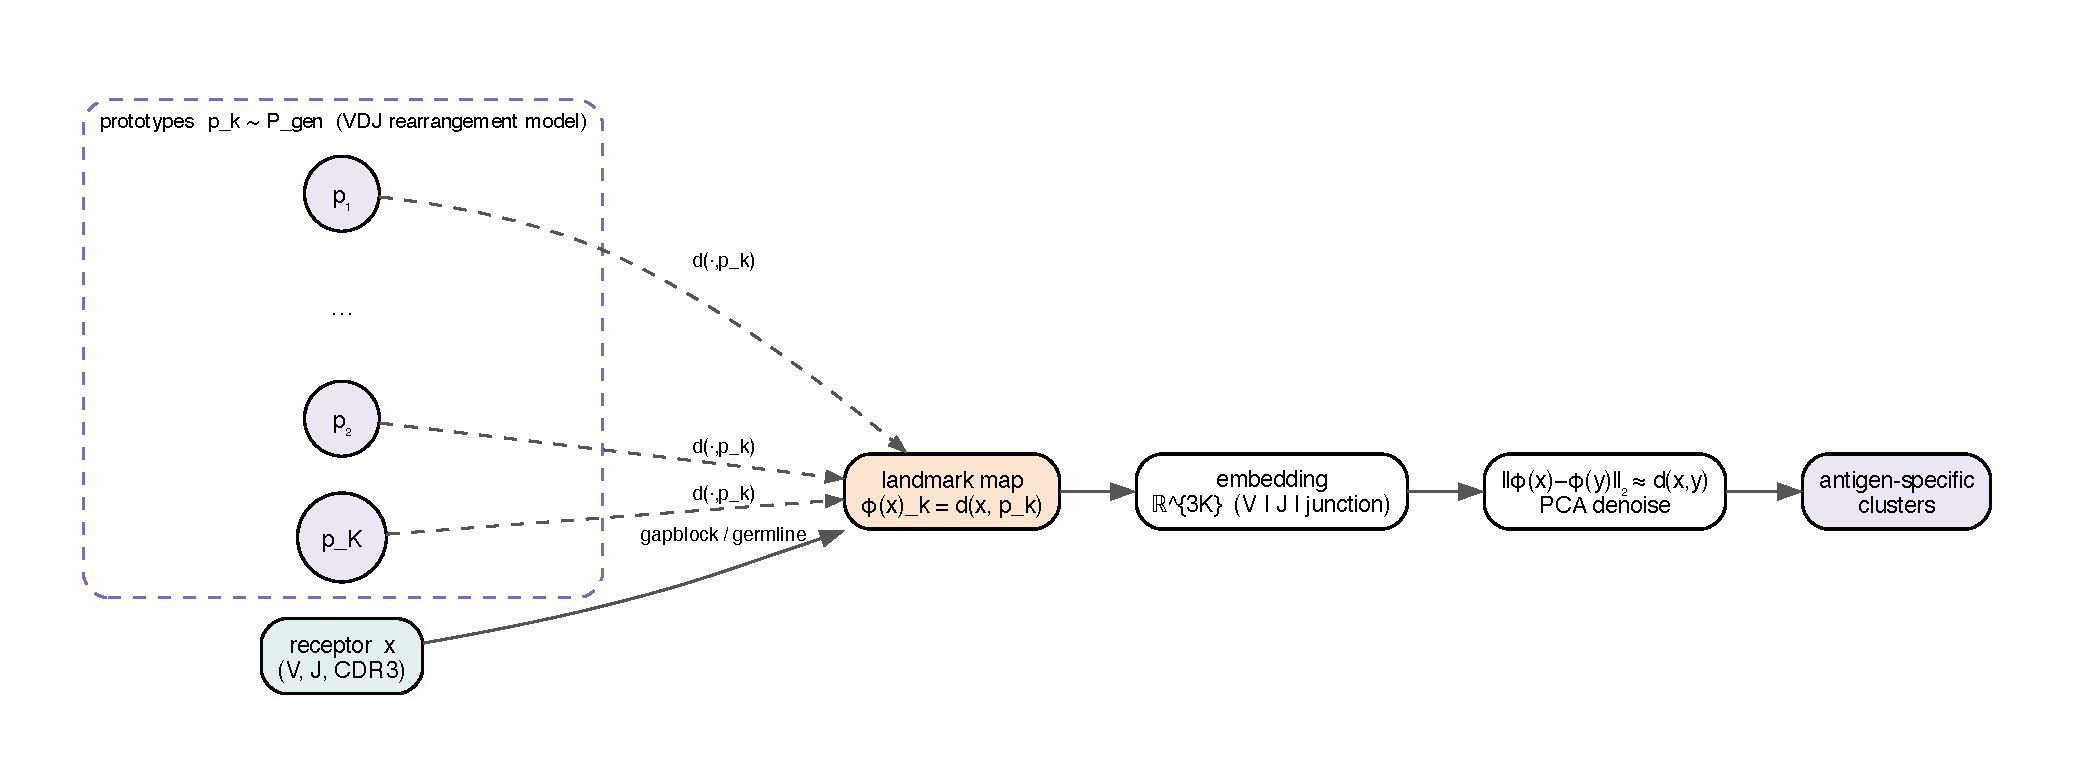
\includegraphics[width=\linewidth]{diagram_embedding.pdf}
  \caption{The {\scshape TCREMP} prototype-embedding pipeline. A receptor $x$ is mapped to the vector of
  its alignment distances to prototypes $p_k$ sampled from the recombination model $\Pgen$; Euclidean
  distance in the resulting $\R^{3K}$ coordinate system approximates pairwise alignment distance
  (Prop.~\ref{prop:lipschitz}--\ref{prop:energy}), and specificity groups become compact clusters.}
  \label{fig:schematic}
\end{figure}

\paragraph{Non-expansiveness} The single structural fact from which everything else follows is that each
coordinate of $\varphi$ is $1$-Lipschitz.

\begin{proposition}[Lipschitz coordinates and the upper bound]\label{prop:lipschitz}
For every prototype $p$ and all $x,y\in X$, $\lvert d(x,p)-d(y,p)\rvert \le d(x,y)$. Consequently
\begin{equation}\label{eq:upper}
  \norm{\varphi(x)-\varphi(y)}_\infty \;\le\; d(x,y)
  \qquad\text{and}\qquad
  D(x,y)=\norm{\varphi(x)-\varphi(y)}_2 \;\le\; \sqrt{K}\,d(x,y).
\end{equation}
\end{proposition}
\begin{proof}
The triangle inequality gives $d(x,p)\le d(x,y)+d(y,p)$ and $d(y,p)\le d(x,y)+d(x,p)$, so
$\lvert d(x,p)-d(y,p)\rvert\le d(x,y)$. Taking the maximum over $p\in P$ gives the $\ell^\infty$ bound;
summing the squares of $K$ terms each $\le d(x,y)^2$ and taking the root gives the $\ell^2$ bound.
\end{proof}

Proposition~\ref{prop:lipschitz} is the rigorous half of the headline ``embedding distance $\lesssim$
alignment distance'' claim: no pair is ever \emph{farther} apart in embedding space (up to $\sqrt K$)
than its alignment distance. The reverse --- that close-in-embedding implies close-in-alignment --- is
not automatic and is where the prototypes must do work.

\paragraph{Exactness in the limit} With enough prototypes the $\ell^\infty$ bound is tight.

\begin{proposition}[Kuratowski isometry]\label{prop:kuratowski}
If $P=X$ then $\norm{\varphi(x)-\varphi(y)}_\infty = d(x,y)$ for all $x,y$; that is, $\varphi$ is an
isometric embedding of $(X,d)$ into $(\ell^\infty,\norm{\cdot}_\infty)$.
\end{proposition}
\begin{proof}
The upper bound is Prop.~\ref{prop:lipschitz}. For the lower bound take the prototype $p=y$: then
$\lvert d(x,y)-d(y,y)\rvert = d(x,y)$, so the supremum over prototypes is at least $d(x,y)$.
\end{proof}

The construction of Eq.~\eqref{eq:embedding} is thus the Kuratowski/Fr\'echet embedding, and the
supplementary experiments that use the sequences themselves as prototypes (\S S1--S2 of
\cite{Kremlyakova2025}) are exactly this isometric regime, read out in $\ell^2$ rather than $\ell^\infty$.
Passing from $\ell^\infty$ to $\ell^2$ costs the $\sqrt K$ factor of Eq.~\eqref{eq:upper} but makes the
coordinates amenable to {\scshape PCA} and Euclidean clustering.

\paragraph{Why $\ell^2$ distance tracks alignment distance} Fix a prototype-sampling measure $\mu$ on
$X$ (in {\scshape TCREMP}, $\mu=\Pgen$) and draw $p_1,\dots,p_K$ i.i.d.\ from $\mu$.

\begin{proposition}[Energy functional]\label{prop:energy}
Define the $\mu$-energy dissimilarity
$\bar D_\mu^2(x,y) \coloneqq \E_{p\sim\mu}\!\bigl[(d(x,p)-d(y,p))^2\bigr]$. Then
$\tfrac1K D(x,y)^2 \to \bar D_\mu^2(x,y)$ almost surely as $K\to\infty$, and $\bar D_\mu^2$ is a
$\mu$-dependent (semi)metric with $0\le\bar D_\mu^2(x,y)\le d(x,y)^2$.
\end{proposition}
\begin{proof}
$\tfrac1K D^2 = \tfrac1K\sum_k (d(x,p_k)-d(y,p_k))^2$ is an empirical mean of i.i.d.\ terms bounded by
$d(x,y)^2$ (Prop.~\ref{prop:lipschitz}); the strong law gives the limit and the bound, and symmetry
plus the triangle inequality for $\norm{\cdot}_2$ make $\bar D_\mu$ a semimetric.
\end{proof}

Proposition~\ref{prop:energy} says $D$ estimates a fixed monotone-in-$d$ functional $\bar D_\mu$: two
receptors that are close under $d$ have similar distance profiles to the whole of $\mu$ and hence small
$\bar D_\mu$, while dissimilar receptors have systematically different profiles. This is the mechanism
behind supplementary Fig.~S2 --- the empirical Pearson correlation between $D_{ij}$ and $d_{ij}$
(Fig.~\ref{fig:s2}, $R=0.64$ under Smith--Waterman, $0.49$ under the \code{gapblock} metric of
\S\ref{sec:metric}) --- and behind S2c/d, where $D_{ik}$ concordates with means of $d_{ik}$ over the
prototype set: those means are Monte-Carlo estimates of $\bar D_\mu$.

\begin{figure}[t]
  \centering
  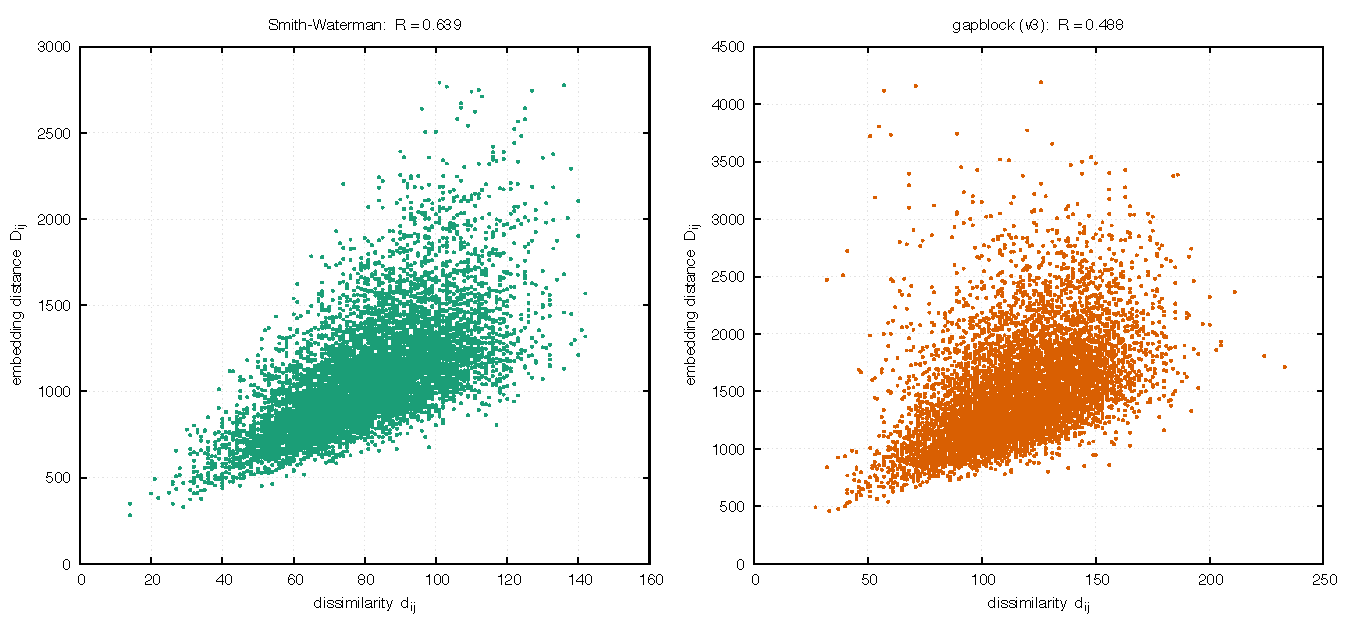
\includegraphics[width=\linewidth]{fig_s2_correlation.pdf}
  \caption{Embedding-space Euclidean distance $D_{ij}$ against pairwise dissimilarity $d_{ij}$ for
  $n=2500$ CDR3$\beta$ used as their own prototypes (Prop.~\ref{prop:energy}; reproduces suppl.\ S2).
  Left: Smith--Waterman $d$; right: the \code{gapblock} metric shipped in v3. Generated by
  \code{mir/bench/theory.py::s2\_dissimilarity\_distance\_correlation}.}
  \label{fig:s2}
\end{figure}

\paragraph{How many prototypes} The $\sqrt K$ gap of Eq.~\eqref{eq:upper} is worst-case; for the
\emph{random} landmark map the relative fluctuation of $\tfrac1K D^2$ around $\bar D_\mu^2$ is
$O(K^{-1/2})$ by Prop.~\ref{prop:energy}, so a Johnson--Lindenstrauss-style argument
\cite{JohnsonLindenstrauss1984} on the bounded coordinates gives the following.

\begin{proposition}[Landmark sample complexity]\label{prop:samplecomplexity}
Let $S\subset X$ with $\lvert S\rvert=n$. For $K = O(\varepsilon^{-2}\log n)$ i.i.d.\ prototypes, with
high probability every pair $x,y\in S$ satisfies
$\bigl\lvert \tfrac1K D(x,y)^2 - \bar D_\mu^2(x,y)\bigr\rvert \le \varepsilon\,d(x,y)^2$ simultaneously.
\end{proposition}
\begin{proof}
Fix a pair $x,y\in S$. Prototype $p_k\sim\mu$ contributes $Y_k=(d(x,p_k)-d(y,p_k))^2$, and the reverse
triangle inequality gives $0\le Y_k\le d(x,y)^2$, so the $Y_k$ are i.i.d.\ and confined to an interval of
length $d(x,y)^2$ with mean $\E_\mu[Y]=\bar D_\mu^2(x,y)$ (Prop.~\ref{prop:energy}). Their average is
$\tfrac1K\sum_k Y_k=\tfrac1K D(x,y)^2$, so Hoeffding's inequality yields
$\Pr\!\big[\lvert\tfrac1K D(x,y)^2-\bar D_\mu^2(x,y)\rvert>\varepsilon\,d(x,y)^2\big]\le2\exp(-2K\varepsilon^2)$.
A union bound over the $\binom n2<n^2$ pairs caps the total failure probability at $2n^2\exp(-2K\varepsilon^2)$,
which tends to $0$ as soon as $K\ge C\varepsilon^{-2}\ln n$, i.e.\ $K=\Theta(\varepsilon^{-2}\log n)$.
\end{proof}

The logarithmic dependence on $n$ is the theoretical counterpart of supplementary Fig.~S4, where the
{\scshape UMAP} of an antigen-specific set stabilises once $K\gtrsim 100$ prototypes are used: the
embedding geometry saturates at a prototype count that grows only logarithmically with the data.
Prototype embeddings are the $\emph{empirical}$ / Nystr\"om feature map of the alignment kernel, and
Landmark {\scshape MDS} \cite{deSilvaTenenbaum2004,FaloutsosLin1995} and the dissimilarity representation
\cite{PekalskaDuin2005} are the classical instances; the {\scshape PCA} step of \S\ref{sec:tcr} is
Landmark {\scshape MDS} on $\varphi$.

\section{The alignment dissimilarity as a metric}\label{sec:metric}

\paragraph{The Gram construction} {\scshape TCREMP} scores two sequences by an alignment similarity $s$
and converts it to a dissimilarity by
\begin{equation}\label{eq:gram}
  d(a,b) = s(a,a) + s(b,b) - 2\,s(a,b).
\end{equation}
This is exactly the squared distance $\norm{\psi(a)-\psi(b)}^2$ induced by a feature map $\psi$ whenever
$s$ is an inner product, $s(a,b)=\langle\psi(a),\psi(b)\rangle$. The v3 implementation
(\code{mir/distances/junction.py}) reads $d$ off directly: \code{seqtree}'s \code{blosum62()} is already
the Gram transform of Eq.~\eqref{eq:gram}, and \code{gapblock.score\_matrix} returns $d$ as a genuine
metric (zero diagonal, symmetric, non-negative), selecting the best of contiguous gap-block placements
at offsets $(3,4,-4,-3)$.

\begin{definition}
A symmetric $d$ with zero diagonal is of \emph{negative type} (equivalently, $-d$ is conditionally
positive definite) if $\sum_{i,j} c_i c_j\, d(x_i,x_j)\le 0$ for all finite $\{x_i\}$ and all
$\{c_i\}$ with $\sum_i c_i = 0$.
\end{definition}

\begin{proposition}[When Eq.~\eqref{eq:gram} is an honest distance]\label{prop:schoenberg}
$d$ of Eq.~\eqref{eq:gram} is of negative type if and only if the centred similarity matrix
$s$ is positive semidefinite, in which case $\sqrt d$ embeds isometrically into a Hilbert space
and $d=\norm{\psi(\cdot)-\psi(\cdot)}^2$ for the associated feature map $\psi$.
\end{proposition}
\begin{proof}
Suppose $d$ is of negative type. Fix a base point $x_0$ and form the centred kernel
$\tilde s(a,b)=\tfrac12\big(d(a,x_0)+d(b,x_0)-d(a,b)\big)$. Given any coefficients $c_1,\dots,c_m$, set
$c_0=-\sum_{i\ge1}c_i$ so that $\sum_{i\ge0}c_i=0$; expanding, $\sum_{i,j\ge1}c_ic_j\,\tilde s(x_i,x_j)
=-\tfrac12\sum_{i,j\ge0}c_ic_j\,d(x_i,x_j)\ge0$ by negative type, so $\tilde s$ is positive semidefinite. As a
PSD kernel $\tilde s$ is a Gram matrix, $\tilde s(a,b)=\langle\psi(a),\psi(b)\rangle$ for a Hilbert-space map
$\psi$, and $\norm{\psi(a)-\psi(b)}^2=\tilde s(a,a)+\tilde s(b,b)-2\tilde s(a,b)=d(a,b)$, so $\sqrt d$ embeds
isometrically. Expanding this square is Eq.~\eqref{eq:gram} with $s(a,b)=\langle\psi(a),\psi(b)\rangle$,
identifying negative type of $d$ with positive semidefiniteness of the centred similarity. Conversely, if $s$
is PSD then Eq.~\eqref{eq:gram} is manifestly a squared Hilbert distance, hence of negative type. This is
Schoenberg's theorem \cite{Schoenberg1938}; \cite{NegativeTypeHilbert2023,CNDkernels2013} give bi-Lipschitz
refinements.
\end{proof}

\paragraph{Alignment scores need correction} General pairwise-alignment similarities (Smith--Waterman,
BLAST) are \emph{not} positive semidefinite, so Eq.~\eqref{eq:gram} can violate $d\ge 0$ or the triangle
inequality; canonicalising an alignment score into a metric requires an explicit correction
\cite{BlastMetric2025}. In v3 this correction is the non-negativity clamp inside \code{seqtree}'s Gram
transform --- a projection of the score onto the nearest conditionally-negative-definite cone --- which
guarantees the metric axioms Prop.~\ref{prop:lipschitz}--\ref{prop:kuratowski} rely on. The choice of
$s$ (BLOSUM62 here; \textsc{tcrBLOSUM} or a {\scshape VDJ}-specific matrix are alternatives) selects
\emph{which} metric; all are admissible provided the clamp restores negative type.

\paragraph{Gap-block versus Smith--Waterman} The v3 junction metric replaces a full Smith--Waterman
optimisation by the best of four predetermined contiguous gap-block placements. When the optimal CDR3
alignment inserts a single contiguous gap inside the hypervariable core --- the generic case once the
conserved Cys/Phe anchors are fixed --- the gap-block score equals the Smith--Waterman optimum; the two
diverge only for multi-gap alignments of very unequal lengths. Empirically the induced coordinate systems
are strongly but not perfectly aligned (Fig.~\ref{fig:s2}: the same $D$--$d$ correlation is $R=0.64$ for
Smith--Waterman and $R=0.49$ for \code{gapblock}), so v3 embeddings are a \emph{new, versioned}
coordinate system rather than a bit-for-bit reproduction of the published one.

\section{Immune receptors and the recombination model}\label{sec:immune}

\paragraph{The prototype measure is $\Pgen$} The diversity of an immune repertoire is astronomically
large, but it is not arbitrary: it is the image of a low-entropy stochastic process, the V(D)J
recombination model $\Pgen$ \cite{Murugan2012,Marcou2018,Sethna2019}. {\scshape TCREMP} takes the
prototype-sampling measure of \S\ref{sec:foundations} to be exactly this model, so each coordinate
$\varphi(x)_k = d(x,p_k)$, $p_k\sim\Pgen$, measures the alignment distance from $x$ to a typical product
of recombination.

\begin{proposition}[Distance-profile functional]\label{prop:profile}
For $p\sim\Pgen$ the empirical distribution of $\{\varphi(x)_k\}_{k=1}^K$ converges weakly to the law of
$d(x,p)$. Hence $\varphi(x)$ is a Monte-Carlo sketch of the map $x\mapsto \mathrm{Law}_{\,p\sim\Pgen}\,
d(x,p)$, and two receptors with the same distance-profile-to-$\Pgen$ are asymptotically
embedding-indistinguishable.
\end{proposition}
\begin{proof}
The coordinates are i.i.d.\ evaluations of the fixed $1$-Lipschitz map $p\mapsto d(x,p)$ under $\Pgen$;
the Glivenko--Cantelli theorem gives uniform convergence of their empirical law to that of $d(x,p)$.
\end{proof}

This reframes what the embedding ``learns'': not a language model of receptor sequences --- which the
entropy of $\Pgen$ ($\sim\!40$ bits for {\scshape TRB}) makes futile --- but each receptor's geometric
relationship to the generative distribution itself. It also predicts that the embedding is insensitive
to how the prototypes are obtained, provided they cover the same support.

\begin{proposition}[Prototype-source robustness]\label{prop:robust}
Let $\mu,\nu$ be two prototype measures that are mutually absolutely continuous with bounded density
ratio $\rho = d\mu/d\nu$ on the support of the repertoire. Then the energy dissimilarities of
Prop.~\ref{prop:energy} satisfy $\bar D_\mu^2(x,y) = \E_{\nu}[\rho(p)\,(d(x,p)-d(y,p))^2]$, so the two
embeddings induce distances that agree up to the $\chi^2$ discrepancy between $\mu$ and $\nu$; as
$\chi^2(\mu\,\Vert\,\nu)\to 0$ the pairwise-distance vectors become perfectly correlated.
\end{proposition}
\begin{proof}
By Prop.~\ref{prop:energy}, $\bar D_\mu^2(x,y)=\E_\mu[u_{xy}(p)]$ with $u_{xy}(p)=(d(x,p)-d(y,p))^2$. Writing
the $\mu$-expectation as a $\nu$-expectation with importance weight $\rho=d\mu/d\nu$ gives
$\bar D_\mu^2(x,y)=\E_\nu[\rho(p)\,u_{xy}(p)]$, the first claim. Its discrepancy from the $\nu$-embedding is
$\bar D_\mu^2-\bar D_\nu^2=\E_\nu[(\rho-1)\,u_{xy}]$, and Cauchy--Schwarz bounds this by
$\sqrt{\E_\nu[(\rho-1)^2]}\,\sqrt{\E_\nu[u_{xy}^2]}=\sqrt{\chi^2(\mu\Vert\nu)}\,\sqrt{\E_\nu[u_{xy}^2]}$, using
$\E_\nu[(\rho-1)^2]=\E_\nu[\rho^2]-1=\chi^2(\mu\Vert\nu)$. Hence the two families of pairwise distances differ
by a factor set by $\chi^2(\mu\Vert\nu)$; as $\chi^2(\mu\Vert\nu)\to0$ the perturbation vanishes uniformly and
their correlation tends to one.
\end{proof}

A real healthy-donor repertoire (Britanova \emph{et al.} \cite{Britanova2016}) and the synthetic
recombination model (Murugan \emph{et al.} \cite{Murugan2012}) are, after thymic selection, close in
exactly this sense, which is why supplementary Fig.~S3 finds their embedding distances correlated at
$R=0.96$ --- reproduced here at $R=0.97$ (Fig.~\ref{fig:s3}).

\begin{figure}[t]
  \centering
  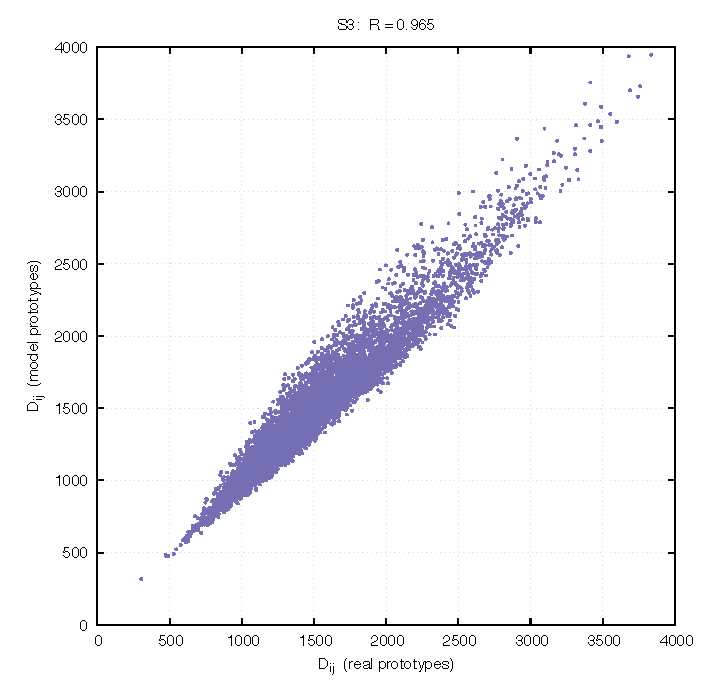
\includegraphics[width=0.52\linewidth]{fig_s3_prototype_source.pdf}
  \caption{Pairwise embedding distances built from real (Britanova \cite{Britanova2016}) versus model
  (OLGA/Murugan \cite{Murugan2012,Sethna2019}) prototypes agree ($R=0.97$; suppl.\ S3), confirming
  Prop.~\ref{prop:robust}. \code{mir/bench/theory.py::prototype\_source\_correlation}.}
  \label{fig:s3}
\end{figure}

\paragraph{Distribution laws} The random construction also fixes the shape of the two histograms that
dominate any embedding analysis.

\begin{proposition}[Dissimilarity and distance laws]\label{prop:laws}
Under mild mixing of per-position alignment contributions: (i) the pairwise dissimilarity $d_{ij}$ is
asymptotically Gamma-distributed --- a sum of many non-negative, bounded per-column penalties, so the
central-limit tendency is tempered by positivity and right-skew; (ii) the embedding distance $D_{ij}$
follows a generalized extreme value (Fr\'echet--Gumbel) law rather than a Gaussian, because
$D=\norm{\varphi(x)-\varphi(y)}_2$ is dominated by its largest coordinate differences, which are
extreme-value statistics over the $K$ prototypes.
\end{proposition}
\begin{proof}
(i) By Eq.~\eqref{eq:gram}, $d(a,b)=\sum_\ell \pi_\ell$ is a sum over aligned columns of bounded, non-negative
Gram penalties $\pi_\ell$. For sequences of comparable length the columns are many and weakly dependent, so a
Lindeberg central-limit tendency applies; but the constraint $d\ge0$ and the bounded support make the limit a
positive, right-skewed law, and among laws on $[0,\infty)$ with matched mean and variance the Gamma family is
the maximum-entropy choice, capturing the skew a Gaussian misses (Fig.~\ref{fig:s1}, left). (ii) The
coordinates of $D(x,y)=\norm{\varphi(x)-\varphi(y)}_2$ are $K$ i.i.d.\ bounded differences
$d(x,p_k)-d(y,p_k)$. Its $\ell^\infty$ part equals $d(x,y)$ (Prop.~\ref{prop:kuratowski}), a maximum over the
$K$ prototypes; by the Fisher--Tippett--Gnedenko theorem \cite{deHaanFerreira2006} the only non-degenerate
limit of a normalised maximum of i.i.d.\ variables is the generalized-extreme-value family, so $D$'s upper
tail is {\scshape GEV}, not Gaussian. In high dimension $\norm{\cdot}_2$ concentrates and its fluctuations are
carried by the same extreme coordinates \cite{Beyer1999}, so the {\scshape GEV} law governs $D$ itself
(Fig.~\ref{fig:s1}, right).
\end{proof}

Both laws are confirmed on v3 (Fig.~\ref{fig:s1}): the Gamma fit to $d_{ij}$ beats the Gaussian on
\textsc{aic}, and the {\scshape GEV} fit to $D_{ij}$ beats the Gaussian decisively
(Kolmogorov--Smirnov $0.021$ versus $0.078$). The fitted shape $\xi\approx 0$ places v3 at the
Gumbel--Fr\'echet boundary, marginally lighter-tailed than the $\xi=+0.11$ of the published
Smith--Waterman construction --- a metric-dependent detail, not a qualitative difference.

\begin{figure}[t]
  \centering
  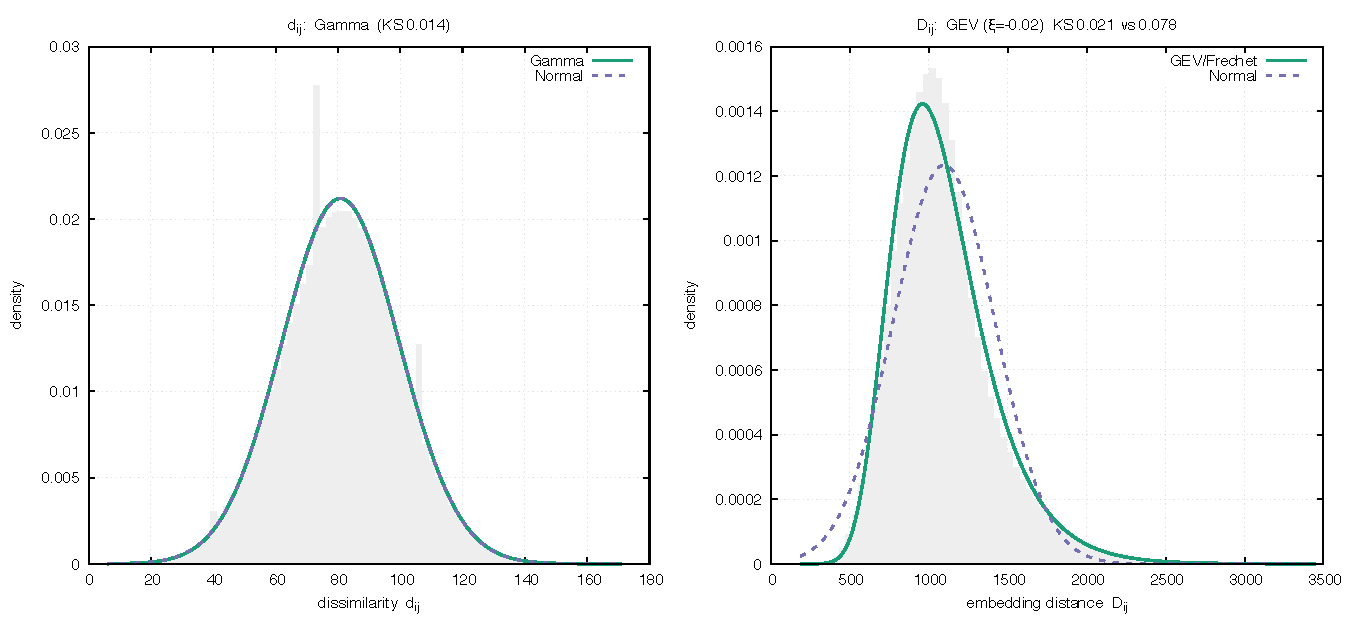
\includegraphics[width=\linewidth]{fig_s1_distributions.pdf}
  \caption{Distribution laws (Prop.~\ref{prop:laws}; suppl.\ S1). Left: $d_{ij}$ is Gamma, not Gaussian.
  Right: $D_{ij}$ follows a {\scshape GEV}/Fr\'echet law (\textsc{ks} $0.021$) that the Gaussian
  ($0.078$) misses on the heavy right tail. \code{mir/bench/theory.py::fit\_distributions}.}
  \label{fig:s1}
\end{figure}

\paragraph{Why not learn the representation?} A natural alternative to Eq.~\eqref{eq:embedding} is to
train a self-supervised sequence model --- a masked or autoregressive ``receptor language model'' --- and
use its latent as the embedding. The recombination model shows why this cannot improve on the alignment
geometry for specificity. Two properties of $\Pgen$ are decisive: it is \emph{low-complexity} and it is
\emph{antigen-blind}.

First, the repertoire process has little learnable structure. $\Pgen$ factorises as a shallow Bayesian
network --- germline gene choice, a nearest-neighbour (dinucleotide Markov) insertion chain, and
independent trimming \cite{Murugan2012,Marcou2018} --- so its \emph{predictive information}, the mutual
information between a CDR3 prefix and its remainder (the excess entropy of the process), is bounded by the
description length of that network: a few bits, and short-range. Natural language carries large predictive
information --- syntax, semantics, world knowledge --- that deep representations discover and compress; a
CDR3 carries almost none beyond its germline templating and local insertion statistics. A likelihood-trained
model therefore converges to a sufficient statistic for $\Pgen$ itself and has nothing further to represent.

Second, and decisively, $\Pgen$ has no antigen variable: generation precedes and is independent of antigen
selection. Let $A$ be the antigen a receptor $X$ recognises, unobserved during self-supervised training.

\begin{proposition}[No unsupervised separation of specificity]\label{prop:nofreelunch}
Let a representation $f$ be fitted by any objective that is a functional of the unlabelled generation
marginal $\Pgen$ alone. Then the training signal carries zero information about the antigen partition,
$I(\text{objective};A)=0$; the population objective is invariant under relabelling of antigens, and the
alignment of $f(X)$ with $A$ is fixed by the inductive bias of $f$ (its architecture, tokenisation, and
metric), not by learning.
\end{proposition}
\begin{proof}
By hypothesis the objective is a functional of the unlabelled generation marginal $\Pgen$ --- equivalently of
the i.i.d.\ sample $X_1,\dots,X_m\sim\Pgen$ --- and never accesses $A$. Because generation precedes selection,
$A$ enters the joint law only through the post-generation selection channel, which the training data do not
observe; hence the training data and $A$ are independent, $I(\text{training data};A)=0$. For any
representation $f$ measurable with respect to that data the data-processing inequality gives
$I(f;A)\le I(\text{training data};A)=0$. The population objective is therefore a functional of $\Pgen$ that
does not reference the antigen partition, so it is invariant under any permutation $\varsigma$ of antigen
labels: if $f^\star$ is optimal, so is $\varsigma\circ f^\star$. No minimiser can prefer an antigen-separating
representation over an antigen-mixing one on the strength of the data, so whatever alignment $f(X)$ has with
$A$ is fixed by the inductive bias of $f$, not learnt.
\end{proof}

Specificity separation in a receptor embedding is thus an \emph{inductive-bias} phenomenon, not a learned
one: it is present exactly insofar as the chosen geometry matches the biophysics of recognition. The
prototype embedding builds in precisely the right bias --- the alignment metric that supplementary Fig.~S5
shows tracks structural (C$\alpha$ {\scshape RMSD}) similarity --- with no training and no antigen labels. A
learned network has only three options: (i) recover $\Pgen$, which does not separate antigens
(Prop.~\ref{prop:nofreelunch}); (ii) be supervised by scarce antigen labels, abandoning the unsupervised
premise and the unlimited $\Pgen$-sampling that makes the approach attractive; or (iii) regress onto the
alignment geometry itself --- which is exactly the Part~2 forward codec (\code{mir/ml/encoder.py}), a network
trained to reproduce $\varphi$. Option (iii) is not a competitor to the prototype embedding but an
accelerator of it: the network learns to \emph{compute} the distance functional quickly, not to discover a
better coordinate, and its embeddings are only as good as the $\varphi$ it approximates. In this precise
sense the alignment-to-reference geometry is the canonical unsupervised coordinate for a repertoire whose
only structure is an antigen-blind generative model, and prototypes are its minimal, assumption-free
realisation.

\paragraph{Specificity is host-conditioned and, in the limit, coverage-complete} Proposition~\ref{prop:nofreelunch}
concerns unlabelled objectives; one might hope to inject the missing antigen signal from a labelled
database. Three facts make even that route converge back to $\Pgen$.

\emph{(1) The label is not a function of the receptor.} What one observes as antigen-specific expansion in a
donor is not a map $X\mapsto$ antigen but the host-restricted shadow $A_h(X)=B(X)\cap(\mathrm{HLA}_h\times
\mathrm{Exposure}_h)$, where $B(X)$ is the large, cross-reactive set of pMHC that $X$ can engage: which
peptides are presented is set by the {\scshape HLA} haplotype, which are encountered by pathogen history.
Both are host latent variables, and donors with identical infections hold sparse, \emph{largely disjoint}
receptor sets that nonetheless cover the same antigens \cite{Mayer2015}. Specificity is thus not a stable,
sequence-intrinsic function: the same $X$ carries different labels in different hosts, so the map is
non-identifiable from sequence across a population.

\emph{(2) Labels cover a vanishing slice.} Databases such as {\scshape VDJdb} \cite{Goncharov2022} annotate
a measure-zero corner of the antigen$\,\times\,$receptor space ($\gtrsim 20^{9}$ peptides per {\scshape MHC}
class, thousands of alleles, $>10^{15}$ possible receptors), so a supervised model saturates at database
coverage and collapses on unseen epitopes --- it learns the covered epitopes, not specificity.

\emph{(3) The completeness limit is $\Pgen$.} Pursuing full coverage does not escape the loop, because the
recombination model is itself the immune system's coverage code: the repertoire is (near-)optimally tuned to
the pathogen distribution, exploiting cross-reactivity so that essentially every antigen has cognate
precursors \cite{Mayer2015,Murugan2012}.

\begin{proposition}[Coverage fixed point]\label{prop:coverage}
Assume coverage-completeness: there is $p_0>0$ such that for almost every antigen $a$,
$\Pr_{x\sim\Pgen}[x\ \text{binds}\ a]\ge p_0$. Then the binding relation is a dense, many-to-many graph
whose antigen-marginal is bounded away from $0$ and $1$ uniformly; averaging the specificity map over the
whole antigen space carries no receptor-discriminative information beyond generation propensity, so as the
labelled antigen set expands to the full space the population optimum of any supervised specificity
representation converges to the antigen-blind $\Pgen$-sufficient statistic of Prop.~\ref{prop:nofreelunch}.
\end{proposition}
\begin{proof}
Coverage-completeness gives $\Pr_{x\sim\Pgen}[x\text{ binds }a]\ge p_0>0$ for almost every antigen $a$, and
cross-reactivity gives the dual bound, each receptor binding a $\Theta(1)$ fraction of $\mathcal A$. Thus the
binding indicator $b(x,a)$ has antigen-marginal $\E_{x\sim\Pgen}[b(x,a)]$ bounded strictly inside $(0,1)$
uniformly in $a$. For any receptor statistic $f(X)$ the specificity information integrated over antigens,
$\int_{\mathcal A} I\big(f(X);b(X,a)\big)\,da$, is then bounded by the entropy of a Bernoulli whose parameter
is pinned away from $0$ and $1$ and whose across-receptor variation is driven by the clone-frequency structure
$\Pgen$ imposes, not by any low-dimensional antigen axis. Hence as the labelled antigen set grows to the whole
space, the population optimum of a supervised specificity representation is determined by generation
propensity alone and converges to the $\Pgen$-sufficient statistic of Prop.~\ref{prop:nofreelunch}.
\end{proof}

The circle closes: an unsupervised model recovers $\Pgen$ and cannot separate antigens
(Prop.~\ref{prop:nofreelunch}); a supervised model learns only its labelled slice (fact 2) of a
host-conditioned, non-identifiable label (fact 1); and the ideal of learning \emph{all} specificity returns
to $\Pgen$ (Prop.~\ref{prop:coverage}), because $\Pgen$ \emph{is} the coverage code. Sampling prototypes from
$\Pgen$ is therefore not an arbitrary reference choice --- it discretises the very coverage design that
antigen breadth is built on, so distance-to-prototypes coordinates a receptor by its position in that
coverage geometry, the maximal host-independent, specificity-relevant structure a sequence can carry.

\section{{\normalfont\scshape TCR}s, three-component embeddings, and paired chains}\label{sec:tcr}

\paragraph{The product metric} {\scshape TCREMP} emits three distances per prototype --- a V-germline, a
J-germline, and a junction distance (or CDR1, CDR2, junction) --- interleaved into $\R^{3K}$
(\code{mir/embedding/tcremp.py}). Writing $\varphi=(\varphi_V,\varphi_J,\varphi_\junc)$ for the three
blocks, the block structure of the Euclidean norm gives the exact decomposition
\begin{equation}\label{eq:product}
  D(x,y)^2 = D_V(x,y)^2 + D_J(x,y)^2 + D_\junc(x,y)^2,
\end{equation}
so the embedding metric is the orthogonal sum of the per-component metrics.

\begin{proposition}[Paired-chain concatenation]\label{prop:paired}
For a paired receptor $(\alpha,\beta)$ embedded by concatenating the per-chain maps,
$D_{\mathrm{pair}}(x,y)^2 = D_\alpha(x,y)^2 + D_\beta(x,y)^2$. More generally, concatenating landmark
embeddings of independent factors realises the $\ell^2$ product of the factor metrics.
\end{proposition}
\begin{proof}
Concatenation stacks coordinate blocks; the squared $\ell^2$ norm of a stacked vector is the sum of the
squared block norms, which is Eq.~\eqref{eq:product} extended across chains.
\end{proof}

Paired $\alpha\beta${\scshape TCR} embedding (suppl.\ S4) and, prospectively, the concatenation of
epitope- and {\scshape MHC}-groove coordinates into a single {\scshape TCR}--pMHC vector are therefore
principled: each modality contributes an orthogonal block and distances add in quadrature.

\paragraph{The germline blocks are low-rank} The V and J coordinates depend on the sequence only through
its germline gene identity, which explains the redundancy that {\scshape PCA} removes.

\begin{proposition}[Germline rank bound]\label{prop:rank}
Let $G_V$ be the number of distinct V alleles present in a dataset $S$. The V-block matrix
$\Phi_V\in\R^{\lvert S\rvert\times K}$ with rows $\varphi_V(x)$ has at most $G_V$ distinct rows, hence
$\operatorname{rank}\Phi_V \le G_V$. The same holds for J with $G_J$, and $G_V,G_J \ll K$.
\end{proposition}
\begin{proof}
$\varphi_V(x)_k = d_V(v(x), v(p_k))$ depends on $x$ only through its V allele $v(x)$ (the germline
distances are a fixed allele$\times$allele table, \code{mir/distances/germline.py}); receptors sharing a
V allele have identical V-rows, so there are at most $G_V$ distinct rows and the rank is bounded by
$G_V$.
\end{proof}

A human {\scshape TRB} repertoire has $G_V\lesssim 60$, $G_J\lesssim 15$, against $K$ in the thousands:
two-thirds of the raw coordinates live in a subspace of dimension $\le G_V+G_J$. The
\code{StandardScaler}$\to$\code{PCA} step (\code{mir/embedding/pca.py}) recovers this compact basis ---
Landmark {\scshape MDS} on $\varphi$ --- and an {\scshape ANOVA} of the leading components against gene
usage recovers the germline axes, while the junction block carries the residual $\Theta(K)$-dimensional
specificity signal.

\paragraph{Structural grounding} That the metric is biologically meaningful, not merely combinatorial, is
shown by supplementary Fig.~S5: embedding distances between {\scshape TCR}:pMHC complexes correlate with
the C$\alpha$ {\scshape RMSD} of their crystal structures. Formally this asserts a Lipschitz map from the
sequence metric $(X,d)$ into the structural metric, so that specificity groups \cite{Glanville2017} ---
receptors binding one epitope --- occupy small-diameter regions of embedding space, and clustering recovers
them (Table~S1;
\code{mir/bench/metrics.py}).

\section{{\normalfont\scshape IGH} and somatic hypermutation}\label{sec:igh}

B-cell receptors differ from {\scshape TCR}s in one decisive respect: after recombination they undergo
somatic hypermutation ({\scshape SHM}), a context-dependent point-mutation process \cite{Yaari2013}.
Write $M_m$ for an operator applying $m$ substitutions to a germline-rearranged sequence.

\begin{proposition}[Bounded embedding drift]\label{prop:drift}
There is a constant $c$ (the maximal per-substitution Gram penalty) such that $d(x,M_m x)\le c\,m$, and
therefore $D(\varphi(x),\varphi(M_m x)) \le \sqrt{K}\,c\,m$. Embedding drift under {\scshape SHM} is
linear in the mutation load $m$.
\end{proposition}
\begin{proof}
Each substitution changes at most one aligned column of Eq.~\eqref{eq:gram}, by at most the bounded
penalty range $c$; $m$ substitutions change $d$ by at most $c\,m$, and Prop.~\ref{prop:lipschitz}
propagates this to $D$ with the $\sqrt K$ factor.
\end{proof}

Proposition~\ref{prop:drift} has two consequences. First, a clonal lineage under affinity maturation
traces a path in embedding space whose step size is set by the per-generation mutation load, so the
embedding preserves lineage proximity --- the substrate for density and trajectory analysis
(\S\ref{sec:density}). Second, it explains why {\scshape IGH} is the hardest chain for the neural codec
of Part~2 (forward cosine $0.79$, exact reconstruction $0.16$, against $\ge0.93$/$0.50$ for {\scshape
TCR}): (i) {\scshape IGH} CDR3s are long, so the fixed-length-40 gap-block tokenisation
(\code{mir/ml/tokenize.py}) truncates an appreciable fraction of the variable middle, discarding
information; (ii) {\scshape SHM} inflates the junction distance by $\Theta(m)$, so germline-rearrangement
prototypes sampled from $\Pgen$ systematically under-cover the mutated support (the density ratio $\rho$
of Prop.~\ref{prop:robust} becomes large and the robustness guarantee degrades); and (iii) the
per-receptor entropy is higher. The remedy the theory suggests is to separate the {\scshape SHM}-robust
germline distance (V/J, Prop.~\ref{prop:rank}) from the mutation-inflated junction distance and to
augment the prototype set with a mutation model, i.e.\ to sample prototypes from $\Pgen$ pushed through
$M_m$ rather than from $\Pgen$ alone.

\section{Density geometry and background subtraction}\label{sec:density}

The embedding turns a repertoire into a point cloud in $\R^{3K}$ (or its {\scshape PCA} projection to
$p\approx65$ coordinates), and the natural null model is the pushforward of the generation measure.
Antigen-driven selection deposits, on top of this null, over-dense \emph{ridges} of convergent receptors;
{\scshape TCRNET} and {\scshape ALICE} \cite{Ritvo2018,Pogorelyy2019,PogorelyyShugay2019} detect
them by counting near-neighbours on a Hamming-$1$ graph. We recast the whole procedure as \emph{density-ratio
estimation} on embedding space --- graph-free --- and give it what an honest treatment requires: a
model of the noise (\S\ref{sec:dens-mix}), the estimator and its rate (\S\ref{sec:dens-dre}), the exact local
test (\S\ref{sec:dens-poisson}--\S\ref{sec:dens-balloon}), calibration of a systematically wrong null
(\S\ref{sec:dens-null}), the differential control that fixes it (\S\ref{sec:dens-diff}), the depth it
requires (\S\ref{sec:dens-depth}), the ridge geometry it estimates (\S\ref{sec:dens-ridge}), and how clone
sizes enter (\S\ref{sec:dens-abund}).

\begin{definition}
Let $f_{\mathrm{gen}} = \varphi_{\#}\Pgen$ be the density of embedded prototypes and $f_{\mathrm{obs}}$
the density of an observed repertoire on embedding space. The \emph{enrichment} is the density ratio
$E(z)=f_{\mathrm{obs}}(z)/f_{\mathrm{gen}}(z)$; convergent selection is the region $E(z)>1$.
\end{definition}

\paragraph{Notation} A receptor (clonotype) $\sigma$ is mapped to a point $z=\varphi(\sigma)\in\R^{p}$ (the
prototype embedding, standardised and {\scshape PCA}-projected to $p\approx65$ coordinates). $\Pgen$ is the
V(D)J generation measure and $\pi_{\mathrm{obs}}$ the sampled-repertoire law; their pushforwards under
$\varphi$ are the densities $f_{\mathrm{gen}}=\varphi_{\#}\Pgen$ and $f_{\mathrm{obs}}=\varphi_{\#}\pi_{\mathrm{obs}}$,
and $E=f_{\mathrm{obs}}/f_{\mathrm{gen}}$ is their ratio. The selection factor $Q(\sigma)\ge0$ reweights
$\Pgen$ into $\pi_{\mathrm{obs}}$ (Eq.~\eqref{eq:selweight}), with normaliser $Z_Q=\E_{\Pgen}[Q]$ and
embedding-space average $q(z)=\E[Q\mid\varphi(\sigma)=z]$. We draw $N$ observed and $M$ background points; a
ball $B(z,r)$ of radius $r$ contains $n_{\mathrm{obs}}$ observed and $n_{\mathrm{bg}}$ background points, with
target null occupancy $\lambda_0=\E[n_{\mathrm{obs}}\mid H_0]$; $r_1$ is the median embedding distance moved by
a single {\scshape CDR3} amino-acid substitution, and $a_j$ (\S\ref{sec:dens-abund}) the read count of
clonotype $j$. Symbols $\E$ (expectation), $\mathrm{Var}$, $\mathrm{CV}=\sqrt{\mathrm{Var}}/\E$, and
$\Phi^{-1}$ (standard-normal quantile) are standard.

\subsection{The repertoire as a mixture, and why the raw \texorpdfstring{$\Pgen$}{Pgen} null is
miscalibrated}\label{sec:dens-mix}

The observed repertoire is not the generation model. A sampled sequence has survived thymic and peripheral
selection, so the observed law is a reweighting of $\Pgen$ \cite{Elhanati2014,Sethna2020},
\begin{equation}\label{eq:selweight}
  \pi_{\mathrm{obs}}(\sigma)=\Pgen(\sigma)\,\frac{Q(\sigma)}{Z_Q},\qquad Z_Q=\E_{\Pgen}[Q],
\end{equation}
with $Q\ge0$ the (non-constant) selection factor; the scalar $Q$ of {\scshape ALICE} is its mean-field
reduction. Let $q(z)=\E[Q(\sigma)\mid\varphi(\sigma)=z]$ be the local mean selection field.

\begin{proposition}[Pushforward ratio is the selection field]\label{prop:selfield}
$E(z)=q(z)/Z_Q$.
\end{proposition}
\begin{proof}
$f_{\mathrm{obs}}(z)=\int\delta(\varphi(\sigma)-z)\,\Pgen(\sigma)Q(\sigma)/Z_Q\,d\sigma
= q(z)\,f_{\mathrm{gen}}(z)/Z_Q$.
\end{proof}

So $E\equiv1$ only if selection is neutral. Two immunological facts make $q$ sharply peaked: \emph{convergent
recombination} makes public receptors recur across individuals in proportion to their generation frequency
\cite{Venturi2006,Quigley2010,Venturi2008}, and \emph{thymic selection} is positively correlated with those
same generation biases \cite{Elhanati2014}, amplifying rather than flattening the hierarchy --- a
rich-get-richer field concentrated on the convergent, germline-proximal support. The cost is a null that is
biased \emph{high} exactly where clones sit.

\begin{proposition}[Size-biased bulk fold; the flood]\label{prop:bulkfold}
Averaging the fold over observed clones,
\begin{equation}\label{eq:cvfold}
  \E_{z\sim f_{\mathrm{obs}}}[E(z)]
  =\frac{\E_{f_{\mathrm{gen}}}[q^2]}{\E_{f_{\mathrm{gen}}}[q]^2}
  =1+\mathrm{CV}^2(q)\;\ge\;1,
\end{equation}
strict whenever $\mathrm{Var}(q)>0$.
\end{proposition}
\begin{proof}
$\E_{f_{\mathrm{obs}}}[E]=\int (q/Z_Q)f_{\mathrm{obs}}=\int(q/Z_Q)^2 f_{\mathrm{gen}}
=\E[q^2]/\E[q]^2=1+\mathrm{Var}(q)/\E[q]^2$.
\end{proof}

A test that assumes $E\equiv1$ therefore rejects across the entire region where $q/Z_Q$ clears the fold
threshold. This is measurable: on a {\scshape VDJdb} benchmark in which known antigen-specific ridges are
admixed with an unrelated repertoire as noise, a raw $\Pgen$ background flags $43\%$ of the noise clones as
``enriched'', whereas a matched control background (\S\ref{sec:dens-diff}) flags only $1\%$ --- a $46$-fold
gain in signal-to-noise. The $43\%$ is the selection inflation $1+\mathrm{CV}^2(q)$, \emph{not} a $43\%$
non-null fraction. The remedy is therefore to recentre the null empirically (\S\ref{sec:dens-null}) or to
cancel $q$ with a matched control (\S\ref{sec:dens-diff}). Note $q/Z_Q$ cannot exceed $1$ everywhere --- both
densities integrate to one, so $\E_{f_{\mathrm{gen}}}[q/Z_Q]=1$ --- so it exceeds $1$ only on the observed
support, which is exactly where clones are tested.

\begin{remark}[Ridges are heterogeneous]\label{rem:ridges}
The signal is a sum of epitope-indexed ridges, $f_{\mathrm{sig}}=\sum_e w_e g_e$, with $w_e=\sum_{\sigma\in
S_e}\pi_{\mathrm{obs}}(\sigma)$ the precursor frequency of epitope $e$; the elevation $g_e/f_{\mathrm{gen}}$ is
\emph{larger} for low-$\Pgen$ (private) motifs at equal observed count. Inheriting the heavy tail of $\Pgen$,
the weights $w_e$ span about two orders of magnitude across epitopes and six within one
\cite{Pogorelyy2018}. The polyclonality of a response tracks this precursor frequency: on {\scshape VDJdb}
the immunodominant HLA-A*02 influenza epitope {\scshape GILGFVFTL} resolves into $32$ distinct convergent
mountains, while the {\scshape CMV} A*02 epitope {\scshape NLVPMVATV} gives only $4$. No global height
threshold separates signal from background across such a range; significance must be assessed locally, and
the constructions below are engineered so that it is.
\end{remark}

\subsection{Enrichment as a density ratio: three estimators and their rate}\label{sec:dens-dre}

Estimating $E$ as a quotient of two kernel-density estimates is doubly bad: it pays the density-estimation
rate twice and blows up where $f_{\mathrm{gen}}$ is small. Direct estimation avoids both, and rests on one
moment identity \cite{Kanamori2009,Sugiyama2012}.

\begin{lemma}[Least-squares characterisation]\label{lem:lsif}
$\E_{f_{\mathrm{gen}}}[g\,E]=\E_{f_{\mathrm{obs}}}[g]$ for all $g\in L^2(f_{\mathrm{gen}})$, and
$E=\arg\min_g\big\{\tfrac12\E_{f_{\mathrm{gen}}}[g^2]-\E_{f_{\mathrm{obs}}}[g]\big\}$.
\end{lemma}
\begin{proof}
$\int g(f_{\mathrm{obs}}/f_{\mathrm{gen}})f_{\mathrm{gen}}=\int g\,f_{\mathrm{obs}}$; the objective equals
$\tfrac12\E_{f_{\mathrm{gen}}}[(g-E)^2]$ up to a constant, minimised uniquely at $g=E$.
\end{proof}

Because the empirical objective uses the two clouds only through sample means, the same target admits three
consistent estimators. \textbf{(i)~Balloon} count-ratio (\S\ref{sec:dens-balloon}), local and carrying an
exact test. \textbf{(ii)~Relative ratio} (RuLSIF) $E_\alpha=f_{\mathrm{obs}}/(\alpha
f_{\mathrm{obs}}+(1-\alpha)f_{\mathrm{gen}})\in[0,1/\alpha]$, fit in a kernel basis \cite{Yamada2013}; it is
bounded, hence valley-stable, and inverts to $E=(1-\alpha)E_\alpha/(1-\alpha E_\alpha)$, with $\alpha$ the
water level --- a denominator denser than $f_{\mathrm{gen}}$ caps the runaway public-convergence fold at
$1/\alpha$. \textbf{(iii)~Classifier} logit: labelling observed points $y{=}1$ (prior $\pi=N/(N{+}M)$) and
background $y{=}0$, a calibrated classifier $\eta$ satisfies
\begin{equation}\label{eq:nce}
  \operatorname{logit}\eta(z)=\log E(z)+\log\tfrac{\pi}{1-\pi}
  \;\cite{Menon2016,GutmannHyvarinen2012},
\end{equation}
so any discriminator --- featurised by the forward codec $\varphi$ of Part~2 (\code{mir/ml/encoder.py}) ---
recovers $\log E$ up to the known imbalance offset and scales to $10$--$100$M receptors; normalising flows
\cite{Papamakarios2021} give the two densities explicitly when wanted. The shared offset $\log(N/M)$ is why
the control-background and $\Pgen$-background detectors estimate the \emph{same} object (\S\ref{sec:dens-poisson}).

\begin{proposition}[Direct estimation beats plug-in]\label{prop:drerate}
If $E$ is bounded and lies in a class of bracketing entropy $H(\varepsilon)\asymp\varepsilon^{-2\gamma}$,
$0<\gamma<1$, the regularised least-squares estimator attains
$\norm{\hat E-E}_{L^2(f_{\mathrm{gen}})}=O_p\!\big(n^{-1/(2+2\gamma)}\big)$, $n=\min(N,M)$, which is minimax
for the likelihood ratio \cite{Nguyen2010}; the plug-in quotient pays the density-estimation rate
$n^{-s/(2s+d)}$ per factor plus a small-denominator variance blow-up.
\end{proposition}
\begin{proof}
By Lemma~\ref{lem:lsif} the population risk of any candidate $g$ is
$J(g)=\tfrac12\E_{f_{\mathrm{gen}}}[(g-E)^2]$ up to an additive constant, so the excess risk of the empirical
minimiser $\hat E$ over a class $\mathcal G$ equals $\tfrac12\norm{\hat E-E}_{L^2(f_{\mathrm{gen}})}^2$.
Empirical-process theory bounds this by an approximation term (the regularisation bias) plus a stochastic
term set by the local modulus of the empirical process indexed by $\mathcal G$, i.e.\ by the entropy integral
$\int_0^\delta\!\sqrt{H(\varepsilon)}\,d\varepsilon\asymp\delta^{1-\gamma}$ when
$H(\varepsilon)\asymp\varepsilon^{-2\gamma}$. Choosing the regularisation so that bias and stochastic term are
of the same order and solving the resulting fixed point for the critical radius $\delta$ gives
$\delta\asymp n^{-1/(2+2\gamma)}$; a matching lower bound follows from Fano's inequality on a $\delta$-packing
of $\mathcal G$, so the rate is minimax \cite{Nguyen2010}. Boundedness of $E$ keeps the class envelope finite
in $L^\infty(f_{\mathrm{gen}})$, which the bound requires. The plug-in quotient
$\hat f_{\mathrm{obs}}/\hat f_{\mathrm{gen}}$ has no such envelope: where $\hat f_{\mathrm{gen}}\!\to\!0$ the
ratio's variance diverges --- exactly the instability the bounded relative ratio $E_\alpha\le1/\alpha$ of
\S\ref{sec:dens-dre} removes by construction.
\end{proof}

At $p\approx65$ the nonparametric rate is slow; treat $\hat E$ as a locally smoothed, not pointwise-exact,
field. The three estimators cross-validate: the classifier gives a fast global $E$, the balloon supplies
calibrated significance, the relative estimator delineates smooth ridge boundaries; disagreement flags
estimation error, not signal.

\subsection{Local significance: the exact point-process test}\label{sec:dens-poisson}

Model the two clouds as independent Poisson point processes of intensities $Nf_{\mathrm{obs}}$,
$Mf_{\mathrm{gen}}$ \cite{Kingman1993}. In a ball $B=B(z,r)$ the counts are Poisson with means
$\int_B Nf_{\mathrm{obs}}$, $\int_B Mf_{\mathrm{gen}}$, independent across disjoint sets (Kingman restriction).

\begin{proposition}[Poisson exact test --- {\scshape ALICE}]\label{prop:poissontest}
Under $H_0:f_{\mathrm{obs}}=f_{\mathrm{gen}}$, with the leave-one-out, Laplace-smoothed null mean
\begin{equation}\label{eq:mu0}
  \mu_0=\frac{(N-1)(n_{\mathrm{bg}}+1)}{M+1},\qquad
  p=\Pr[\mathrm{Poisson}(\mu_0)\ge n_{\mathrm{obs}}],
\end{equation}
the enrichment $p$-value is exact given $\mu_0$; for an empty background ball the rule-of-three bound
$\mu_0=3N/M$ applies. This is \eqref{eq:mu0} as implemented in \code{mir/density.py}.
\end{proposition}
\begin{proof}
Poisson tail on the restricted process; $(N-1)/(M+1)$ with $+1$ in the numerator is the rule-of-succession
($\mathrm{Beta}(1,1)$) estimate of the ball probability with self-exclusion, and $3N/M$ is the $95\%$ upper
bound on a Poisson mean from zero events.
\end{proof}

\begin{proposition}[Conditional binomial --- {\scshape TCRNET}]\label{prop:ctest}
For independent processes with in-ball means $\mu_{\mathrm{obs}},\mu_{\mathrm{bg}}$, conditioning on the total
$T=n_{\mathrm{obs}}+n_{\mathrm{bg}}$ gives
$n_{\mathrm{obs}}\mid T\sim\mathrm{Binomial}(T,\mu_{\mathrm{obs}}/(\mu_{\mathrm{obs}}+\mu_{\mathrm{bg}}))
\xrightarrow{H_0}\mathrm{Binomial}(T,N/(N{+}M))$, the local volume cancelling. This nuisance-free two-sample
test \cite{Krishnamoorthy2004} is the binomial branch used with a real control background.
\end{proposition}

\begin{proposition}[{\scshape ALICE} is the rare-event limit of {\scshape TCRNET}]\label{prop:alicelim}
With $p_{\mathrm{bg}}=(n_{\mathrm{bg}}{+}1)/(M{+}1)\sim\lambda_0/M\ll1$, the Le~Cam / Chen--Stein bound
\cite{Arratia1990} gives
$d_{\mathrm{TV}}\big(\mathrm{Binomial}(T,p_{\mathrm{bg}}),\mathrm{Poisson}(Tp_{\mathrm{bg}})\big)\le
Tp_{\mathrm{bg}}^2$, so the two exact tests agree to $O(\lambda_0 p_{\mathrm{bg}})$.
\end{proposition}

Proposition~\ref{prop:alicelim} is the theoretical reason a generated $\Pgen$ background (Poisson) and a real
control (binomial) return the \emph{same} enriched set --- benchmarked at Jaccard $0.86$ against a chance
$0.30$; {\scshape ALICE} is a special case of {\scshape TCRNET}, and the residual $0.14$ is the
convergence-field over-call the differential control removes (\S\ref{sec:dens-diff}). One caveat: clonal
expansion makes raw counts super-Poisson, so counting must be over \emph{distinct} clonotypes and the null
recentred (\S\ref{sec:dens-null}).

\subsection{The balloon estimator and the detection floor}\label{sec:dens-balloon}

Set the radius $R(z)$ to the distance to the $k$-th \emph{background} neighbour, $k=\mathrm{round}(\lambda_0
M/N)$. The shared ball volume cancels from the ratio, which is what makes the estimator usable in high
dimension \cite{Loftsgaarden1965,Terrell1992,BiauDevroye2015}.

\begin{proposition}[Volume-free ratio; homogenised null]\label{prop:balloon}
The balloon densities $\hat f_{\mathrm{obs}}=n_{\mathrm{obs}}/(N V_pR^p)$,
$\hat f_{\mathrm{gen}}=n_{\mathrm{bg}}/(M V_pR^p)$ give
\begin{equation}\label{eq:volfree}
  \hat E(z)=\frac{n_{\mathrm{obs}}/N}{n_{\mathrm{bg}}/M},\qquad
  k=\mathrm{round}\!\big(\lambda_0 M/N\big)\ \Longrightarrow\ \E[n_{\mathrm{obs}}\mid H_0]\approx\lambda_0
  \ \text{for all }z.
\end{equation}
The null is $\mathrm{Poisson}(\lambda_0)$ independent of the local density $f_{\mathrm{gen}}(z)$; the leading
rate is set by the intrinsic dimension $d^\ast\ll p$ of the receptor manifold, not by $p$.
\end{proposition}
\begin{proof}
Fixing $k$ background points fixes the enclosed background mass $\approx k/M$, so the expected observed count
is $N\!\cdot\!k/M=\lambda_0$; $V_pR^p$ cancels between numerator and denominator, removing the explicit
dimension.
\end{proof}

Fixing $\lambda_0$ (rather than the radius) is exactly what Remark~\ref{rem:ridges} demands: with precursor
frequencies spanning orders of magnitude, a fixed radius would be empty in sparse regions and saturated in
dense ones, whereas fixing the null occupancy makes every ball testable on its own scale.

\begin{proposition}[Minimum detectable enrichment]\label{prop:mindetect}
Under $H_1$ with local fold $E$, $n_{\mathrm{obs}}\sim\mathrm{Poisson}(E\lambda_0)$, and a one-sided level-$q$
test is cleared at $50\%$ power once
\begin{equation}\label{eq:estar}
  E^\ast(q,\lambda_0)=1+\frac{c(q)}{\sqrt{\lambda_0}},\qquad c(q)=\Phi^{-1}(1-q);
\end{equation}
under Benjamini--Hochberg over $N$ tests $c\approx\sqrt{2\ln N}$. Thus $E^\ast$ falls only as
$\lambda_0^{-1/2}$ while the radius grows as $\lambda_0^{1/d^\ast}$ (essentially flat in high $d^\ast$) and
must stay $\lesssim r_1$, the median one-substitution embedding drift, to resolve a motif ridge; balancing
these gives the default $\lambda_0=3$ (detectable $\sim\!2.3$-fold) with the range $[1,5]$.
\end{proposition}
\begin{proof}
By Proposition~\ref{prop:balloon} the null count is $n_{\mathrm{obs}}\sim\mathrm{Poisson}(\lambda_0)$, of mean
and variance $\lambda_0$. The one-sided level-$q$ test rejects at $n_{\mathrm{obs}}\ge\tau_q$ with
$\tau_q=\min\{k:\Pr[\mathrm{Poisson}(\lambda_0)\ge k]\le q\}$, and the normal approximation gives
$\tau_q\approx\lambda_0+c(q)\sqrt{\lambda_0}$, $c(q)=\Phi^{-1}(1-q)$. Under $H_1$ the count has mean
$E\lambda_0$, so the test attains $50\%$ power once $E\lambda_0\ge\tau_q$, i.e.\ once
$E\ge1+c(q)/\sqrt{\lambda_0}$ --- Eq.~\eqref{eq:estar}. Demanding power $1-\beta$ replaces $c(q)$ by
$c(q)+\Phi^{-1}(1-\beta)$, and under Benjamini--Hochberg the effective per-test level tightens to $\approx
q/N$, whence $c\approx\Phi^{-1}(1-q/N)\approx\sqrt{2\ln N}$. The exact Poisson tail at $q{=}0.05$ has critical
counts $\tau=4,7,10$ for $\lambda_0=1,3,5$, giving $E^\ast=\tau/\lambda_0\approx4.0,2.3,2.0$. Finally a ball
holding $\lambda_0$ of the $M$ background points encloses mass $\lambda_0/M\propto R^{d^\ast}$ on the
intrinsic-dimension-$d^\ast$ manifold, so $R\propto\lambda_0^{1/d^\ast}$ --- nearly flat for large $d^\ast$,
so raising $\lambda_0$ costs almost no resolution until $R$ reaches the motif width $r_1$, which pins the
operating point at $\lambda_0=3$.
\end{proof}

Pinning $R\approx r_1$ makes the ball the continuous analogue of the Hamming-$1$ shell, and $E(z)$ is its
$r\to0$ limit, $E(z)=\lim_{r\to0}\big[n_{\mathrm{obs}}(B_r)/(N{-}1)\big]/\big[n_{\mathrm{bg}}(B_r)/M\big]$.
This explains the measured continuous--discrete concordance: the Spearman correlation between the balloon
count and the discrete Hamming-$1$ count is $\rho=0.37,0.34,0.11,-0.05$ at $r=0.5,1,2,3\times r_1$ --- high
at one substitution (where the ball coincides with the graph neighbourhood), decaying past it as the ball
integrates several mode basins. The continuous test \emph{generalises} the graph test rather than reproducing
it.

\subsection{Empirical-null calibration: the water level}\label{sec:dens-null}

By Proposition~\ref{prop:bulkfold} the theoretical $\Pgen$ null is wrong by a global factor; before any
multiplicity control it must be recentred to the data. This is Efron's empirical null
\cite{Efron2004}, and it precedes {\scshape FDR}.

\begin{proposition}[Enrichment is an inverse local {\scshape fdr}]\label{prop:localfdr}
In the two-groups model $f=\pi_0 f_0+\pi_1 f_1$ with a \emph{calibrated} null $f_0$, the local false-discovery
rate is $\mathrm{fdr}(z)=\pi_0 f_0(z)/f(z)=\pi_0/E(z)$; declaring $E(z)\ge1/\alpha$ is a conservative
$\mathrm{fdr}\le\alpha$ rule \cite{Efron2004}. With the raw null $f_0=f_{\mathrm{gen}}$ one instead has
$\mathrm{fdr}=\pi_0\mu_0/E$ --- off by the miscalibration of \eqref{eq:cvfold}.
\end{proposition}

\begin{proposition}[Water level $=$ one-sided empirical-null recentring]\label{prop:empnull}
Let the true background be $f_{\mathrm{bg}}(z)=s\,f_{\mathrm{gen}}(z)$ on the tested support with unknown
inflation $s>1$. If the ridge fraction is below $\tfrac12$, then
\begin{equation}\label{eq:waterlevel}
  c=\max\!\Big(\frac{\mathrm{median}_i\,n_{\mathrm{obs},i}}{\mathrm{median}_i\,\mu_{0,i}},\,1\Big),
  \qquad \mu_0\leftarrow c\,\mu_0
  \;\Longrightarrow\; \mathrm{median}_i\,\mathrm{fold}_i\approx1,
\end{equation}
and $c$ is a robust (breakdown $\tfrac12$) consistent estimate of $s$.
\end{proposition}
\begin{proof}
Write $\log\hat E=\log s+\varepsilon$ with $\varepsilon\approx0$ on the bulk and $>0$ on ridges; if ridges
occupy under half the tests, $\mathrm{median}(\log\hat E)=\log s$, so \eqref{eq:waterlevel} estimates $s$ and
$\max(\cdot,1)$ enforces one-sidedness (never deflate below the $\Pgen$ floor). This is Efron's empirical-null
location correction \cite{Efron2004}, equivalently the median-of-ratios size factor of {\scshape DESeq}
\cite{AndersHuber2010}. Being a median it is bounded above by the mean $1+\mathrm{CV}^2(q)$ of
\eqref{eq:cvfold}.
\end{proof}

This is the \code{calibrate="median"} step of \code{mir/density.py}: because the signal is $<\!5\%$ in a naive
repertoire it barely moves the median, so recentring the bulk to fold~$\approx1$ is robust. After recentring,
overlapping balls are positively associated, so Benjamini--Hochberg controls the {\scshape FDR} under
positive-regression dependence \cite{BenjaminiHochberg1995,BenjaminiYekutieli2001}. The failure mode is
sharp: a single scalar $c$ removes only a \emph{constant} inflation. A spatially varying selection field
$s(z)$ --- or a tetramer-sorted sample with ridge fraction $\ge\tfrac12$ --- breaks the median, and the only
fix is a real control.

\subsection{The differential control: cancelling convergence pointwise}\label{sec:dens-diff}

\begin{proposition}[Shared-field cancellation]\label{prop:diffcancel}
Let case and control share the selection/convergence field,
$f_{\mathrm{case}}=(q/Z_Q)f_{\mathrm{gen}}(1+a_1)$ and $f_{\mathrm{ctrl}}=(q/Z_Q)f_{\mathrm{gen}}(1+a_0)$,
with $a_i\ge0$ the condition-specific antigen expansion. Then
\begin{equation}\label{eq:diff}
  R(z)=\frac{f_{\mathrm{case}}(z)}{f_{\mathrm{ctrl}}(z)}=\frac{1+a_1(z)}{1+a_0(z)}
  \;\perp\; q,\,Z_Q,\,f_{\mathrm{gen}},
\end{equation}
independent of the shared field; under $H_0$ ($a_1\equiv a_0$) $R\equiv1$ with \emph{no} water-level offset,
even where $q(z)$ varies spatially. The binomial test of Proposition~\ref{prop:ctest} is its finite-sample
plug-in; {\scshape ALICE} is the special case control~$\equiv f_{\mathrm{gen}}$ after recentring.
\end{proposition}
\begin{proof}
Direct division cancels the shared factor $(q/Z_Q)f_{\mathrm{gen}}$; in the small-ball limit the
case/control odds converge to $(N_{\mathrm{case}}/N_{\mathrm{ctrl}})\,R(z)$, a Radon--Nikodym change of
reference from the generation model to the control.
\end{proof}

\begin{proposition}[Control-absent motifs are maximally identifiable]\label{prop:absent}
If the control lacks a motif on a region $A$ ($f_{\mathrm{ctrl}}\to0$, $f_{\mathrm{sig}}>0$) then
$R\to\infty$ on $A$ (odds-ratio $\to$ relative-risk regime \cite{Cornfield1951}); under the pure-control
anchor $\operatorname{ess\,inf}_z(f_{\mathrm{sig}}/f_{\mathrm{ctrl}})=0$ the mixing weight is identified as
$1-\pi=\operatorname{ess\,inf}_z R(z)$ \cite{Blanchard2010}.
\end{proposition}

This is why the recommended course of action prefers a biological control (pre- vs post-vaccination, patient
vs healthy, {\scshape B27}$\pm$) over the raw $\Pgen$ null, and it is what the benchmarks show. The public
$\texttt{CASSVGL[YF]STDTQYF}$ (TRBV9/TRBJ2-3) motif is control-absent in ankylosing spondylitis, so
$R\to\infty$ on its ridge: it surfaces among enriched {\scshape B27}$+$ synovial hits ($9$) and is absent in
{\scshape B27}$-$ ($0$). In yellow-fever vaccination the shared naive field cancels, isolating the expansion:
day-$15$ versus day-$0$ enriched hits matching the {\scshape LLW}/A*02 reference are $63>35$ (of $129$ vs
$79$ distinct such clonotypes present). Cancellation requires case and control to share $q$ --- match {\scshape
HLA}, depth, and cell subset; a contaminated control attenuates $R$ toward $1$, making the differential test
conservative, not anti-conservative.

\subsection{Sampling depth: why the full repertoire}\label{sec:dens-depth}

Subsampling a repertoire with retention probability $s$ is Poisson thinning: counts scale to
$\mathrm{Poisson}(s\mu)$ \cite{Kingman1993}.

\begin{proposition}[Thinning cost and detection boundary]\label{prop:depth}
With signal mass $\Lambda_e$ and null mean $\lambda_0$, the test's non-centrality
$\delta=\Lambda_e/\sqrt{\lambda_0}$ thins as $\delta_s=\sqrt{s}\,\delta$. Writing depth $D=sN$ and
$\lambda_0\propto Dw_e$, the minimum detectable precursor frequency is
\begin{equation}\label{eq:depthfloor}
  w_e^{\min}(D)=\frac{c(\alpha,\beta,\lambda_0)}{D},
\end{equation}
and a clone is even \emph{observed} only with probability $1-e^{-Dw_e}$ \cite{Good1953}.
\end{proposition}
\begin{proof}
Poisson thinning with retention probability $s$ maps the intensity of every region from $\mu$ to $s\mu$
\cite{Kingman1993}. At depth $D=sN$ a ridge of precursor frequency $w_e$ contributes an expected in-ball
signal count $\propto Dw_e$ against a null of mean $\lambda_0$ and standard deviation $\sqrt{\lambda_0}$, so
by the Gaussian approximation of Proposition~\ref{prop:mindetect} its power is
$\Phi\!\big(Dw_e/\sqrt{\lambda_0}-\Phi^{-1}(1-\alpha)\big)$, reaching $1-\beta$ exactly when
$Dw_e\ge\big(\Phi^{-1}(1-\alpha)+\Phi^{-1}(1-\beta)\big)\sqrt{\lambda_0}$; that is
$w_e\ge w_e^{\min}(D)=c/D$ with $c=\big(\Phi^{-1}(1-\alpha)+\Phi^{-1}(1-\beta)\big)\sqrt{\lambda_0}$, which is
Eq.~\eqref{eq:depthfloor}. Independently, the clone is \emph{present} at all only if its count
$\mathrm{Poisson}(Dw_e)$ is nonzero, an event of probability $1-e^{-Dw_e}$ \cite{Good1953}.
\end{proof}

Antigen clusters are rare in \emph{absolute} number, so subsampling by $s$ inflates the detection floor by
$1/s$ and drops sparse ridges below it --- and at reduced depth low-$w_e$ clusters are often not sampled at
all. Hence the full repertoire must be processed; save memory with junction-only embedding or a {\scshape
PCA}-fit cap, never by subsampling. Because $w_e$ is heavy-tailed (Remark~\ref{rem:ridges}), the boundary
$Dw_e=c$ is crossed at a different depth for every epitope --- one more reason significance is local, never a
global height.

\subsection{Ridge delineation and per-ridge tests}\label{sec:dens-ridge}

The antigen-specific groups are the high components of $E$: its \emph{density ridges}
\cite{Genovese2014} and upper-level-set components \cite{ChaudhuriDasgupta2010,Rinaldo2010}.

\begin{proposition}[Ridge extraction as level-set estimation]\label{prop:ridge}
The connected components of $\{z:E(z)>\tau\}$ form the density cluster tree; distinct epitope motifs are
distinct components appearing at different levels, so no single global $\tau$ certifies all of them, but each
is certified locally. The {\scshape FDR}-significant hit set $\{q<\alpha,\ \mathrm{fold}>1\}$ estimates one
level set, and {\scshape DBSCAN} with $\varepsilon=r_1$, $\mathrm{minPts}\in\{2,3\}$ links its points into
motifs --- its core-point rule is itself a superlevel-set threshold \cite{Ester1996,Rinaldo2010}, so
clustering and the Poisson test stay mutually consistent; $\varepsilon\gg r_1$ over-merges, the same regime
where the continuous--discrete concordance collapses.
\end{proposition}

Each motif is then labelled: a two-sample Poisson test versus a matched control for a condition, and, for an
epitope, the binomial test of \cite{PogorelyyShugay2019} --- successes $=$ receptors in the ridge matching the
epitope, trials $=$ ridge size, probability $=$ the repertoire-wide annotation rate --- with
Benjamini--Hochberg across ridges. Because each ridge is judged against its own local background, the height
heterogeneity of Remark~\ref{rem:ridges} is handled automatically; background subtraction removes the smooth
selection field and the surviving convergent groups are the antigen-specific clusters.

\subsection{Clonal abundance: scoring with clone sizes, robustly}\label{sec:dens-abund}

The tests so far count \emph{distinct} clonotypes, discarding each clone's read count $a_j$. This is
deliberate --- read counts are heavy-tailed (roughly Zipf or log-normal), so a single hyperexpanded clone
would dominate a raw read-weighted count --- but it throws away real signal. Two independent signatures mark
an antigen-driven response: \emph{breadth}, a group of similar sequences produced by convergent
diversification (measured by the neighbour count $n_{\mathrm{obs}}$), and \emph{depth}, a clonotype present at
high copy number through clonal expansion (measured by $a_j$). A textbook antigen-specific cluster shows both,
but the corners matter: a convergent cluster of singletons has breadth without depth, and a hyperexpanded
\emph{orphan} --- large $a_j$, few or no neighbours, the case \cite{PogorelyyShugay2019} recommends inspecting
individually --- has depth without breadth. A complete detector reads both channels, and uses size to boost
the score without letting its tail rule the outcome.

\paragraph{A variance-stabilised weighted count} Replace the in-ball count by a weighted mass
\begin{equation}\label{eq:weighted}
  S(z)=\sum_{j\in B(z,r)} g(a_j),
\end{equation}
with $g$ non-decreasing and \emph{concave} --- for instance $g(a)=\log(1+a)$ or the Anscombe root
$g(a)=\sqrt{a+\tfrac38}$. Concavity is precisely robustness: the leverage of clone $j$ on $S$ is the marginal
$g'(a_j)$, which \emph{decreases} with size, so a size-$1000$ clone amid size-$1$ neighbours contributes a
bounded increment, not a thousandfold one. The endpoints are the read count $g(a)=a$ (constant leverage,
Zipf-dominated) and the shipped distinct count $g(a)=1$ (zero leverage, no size information); $g$ is a tunable
sensitivity--robustness dial between them.

\begin{proposition}[Compound-Poisson null for the weighted count]\label{prop:abund}
Under $H_0$ the in-ball clones are a $\mathrm{Poisson}(\lambda_0)$-sized sample with independent abundances
$A\sim\nu$ (the null size law), so
\begin{equation}\label{eq:abundmoments}
  \E[S\mid H_0]=\lambda_0\,\E_\nu[g(A)],\qquad
  \mathrm{Var}[S\mid H_0]=\lambda_0\,\E_\nu[g(A)^2],
\end{equation}
with dispersion index $\mathrm{Var}/\E=\E_\nu[g(A)^2]/\E_\nu[g(A)]$, equal to $1$ for $g\equiv1$ (a Poisson
null) and $\gg1$ for $g(a)=a$ under a heavy-tailed $\nu$. A negative-binomial (Gamma--Poisson) tail matched to
these two moments gives a calibrated one-sided $p$-value; a variance-stabilising $g$ keeps the null close to
Poisson, so the exact test of \S\ref{sec:dens-poisson} still applies.
\end{proposition}
\begin{proof}
Write $S=\sum_{i=1}^{K}g(A_i)$ with $K\sim\mathrm{Poisson}(\lambda_0)$ and $A_i\sim\nu$ i.i.d.\ and
independent of $K$. Wald's identity gives $\E[S]=\E[K]\,\E[g(A)]$, and the law of total variance gives
$\mathrm{Var}[S]=\E[K]\,\mathrm{Var}[g(A)]+\mathrm{Var}[K]\,\E[g(A)]^2
=\lambda_0\big(\mathrm{Var}[g(A)]+\E[g(A)]^2\big)=\lambda_0\,\E[g(A)^2]$, using
$\E[K]=\mathrm{Var}[K]=\lambda_0$. The dispersion index follows, and for $g\equiv1$ it is $1$, recovering the
$\mathrm{Poisson}(\lambda_0)$ null of Proposition~\ref{prop:balloon}.
\end{proof}

\paragraph{The orphan channel} A hyperexpanded clone with few neighbours is invisible to $S$ yet significant
on its own. Under neutral sampling at depth $D$ its size is $\mathrm{Poisson}(Df_j)$ with $f_j$ its frequency,
so its abundance $p$-value against the null size law,
\begin{equation}\label{eq:orphan}
  p^{\mathrm{size}}_j=\Pr_{A\sim\nu}[A\ge a_j],
\end{equation}
tests expansion independently of any neighbourhood. Combining the breadth and depth channels by Fisher's rule,
$-2\big(\log p^{\mathrm{nbr}}_j+\log p^{\mathrm{size}}_j\big)\sim\chi^2_4$ under the (approximately
independent) null, recovers the orphan when $p^{\mathrm{nbr}}\!\approx\!1$ but $p^{\mathrm{size}}$ is small,
and multiplicatively sharpens a cluster that is both convergent and expanded.

\begin{remark}[Rarefaction sets the size law]\label{rem:rarefaction}
The null size law $\nu$ and the breadth/depth balance are read from the frequency-of-frequencies spectrum ---
the counts $f_1,f_2,\dots$ of singletons, doubletons, and larger clones \cite{Good1953}. The Good--Turing mass
on unseen clones is $\approx f_1/D$, and the singleton fraction is a saturation gauge: a repertoire heavy in
singletons is undersampled, so breadth carries the signal, whereas a saturated repertoire lets depth
dominate. Singletons and doubletons are the convergence substrate; the $3{+}$ and hyperexpanded classes are
where the weight $g$ and the orphan test earn their keep.
\end{remark}

This abundance layer leaves the geometry untouched: $S$ replaces $n_{\mathrm{obs}}$ in the same balloon, the
same recentring (\S\ref{sec:dens-null}) and {\scshape FDR} apply, and the orphan test is a per-clonotype
side-channel. Clone sizes then boost the score exactly where expansion co-occurs with convergence, while the
concavity of $g$ keeps the Zipf tail from ruling the result. The shipped \code{mir/density.py} uses
$g\equiv1$; the weighted and orphan channels are the abundance-aware extension.

\subsection{Course of action}\label{sec:dens-algo}

The theory fixes every parameter, giving a graph-free reincarnation of {\scshape TCRNET}/{\scshape ALICE}
(\code{mir/density.py}):
\begin{enumerate}\itemsep2pt
\item \textbf{Background.} With a matched control, use it and the binomial test
  (Prop.~\ref{prop:diffcancel}); otherwise generate $M\ge5N$ samples from $\Pgen$ and use the Poisson test.
  Prefer a control whenever one exists.
\item \textbf{One basis.} Embed both clouds through one prototype set and one {\scshape PCA} rotation
  (Lemma~\ref{lem:lsif}); $E(z)$ is meaningless across mismatched bases.
\item \textbf{Adaptive ball.} Per observed $z$, radius $=$ distance to the $k$-th background neighbour,
  $k=\mathrm{round}(\lambda_0 M/N)$, $\lambda_0=3$ (Prop.~\ref{prop:balloon},~\ref{prop:mindetect}); count
  $n_{\mathrm{obs}},n_{\mathrm{bg}}$; form $\mu_0$ by \eqref{eq:mu0}.
\item \textbf{Recentre} the $\Pgen$ null by \eqref{eq:waterlevel} (Prop.~\ref{prop:empnull}); a differential
  control needs none.
\item \textbf{Test} the exact upper tail (Poisson or binomial), Benjamini--Hochberg $q<0.05$,
  $\mathrm{fold}>1$; the detection floor is $E^\ast\approx1+c(q)/\sqrt{\lambda_0}$.
\item \textbf{(Optional) clone sizes.} Swap $n_{\mathrm{obs}}$ for the variance-stabilised weighted count
  $S(z)=\sum g(a_j)$ and add the per-clonotype orphan test (\S\ref{sec:dens-abund},
  Prop.~\ref{prop:abund}) to score expansion alongside convergence.
\item \textbf{Cluster} hits by {\scshape DBSCAN}, $\varepsilon=r_1$ (Prop.~\ref{prop:ridge}), and test each
  motif for label enrichment. Process the full repertoire (Prop.~\ref{prop:depth}).
\end{enumerate}
Every default traces to a theorem rather than to tuning; the same estimand $E=f_{\mathrm{obs}}/f_{\mathrm{gen}}$
underlies the graph tests it replaces, the neural classifier of Part~2, and the smooth relative-ratio field.

\section{Privacy: the embedding as a keyed, lossy representation}\label{sec:privacy}

Immune repertoires are individually identifying --- like genomic data, a person's {\scshape TCR}s are a
stable, near-unique fingerprint --- so whether an embedding may be shared in place of raw sequences is a
practical question with a clean geometric answer. Reproducing a coordinate requires two secrets: the
prototype set $P=\{p_k\}$ and the {\scshape PCA} rotation $W$ fitted to the cohort (together with the
centring $\mu$ and scaling). Write the released representation as $Z=(\varphi(X)-\mu)\,W\in\R^{n\times m}$
with $m\ll 3K$.

\paragraph{Three barriers to reconstruction} \emph{(i) Lossy projection.} {\scshape PCA} to $m$ components
discards a $(3K-m)$-dimensional subspace, so $\varphi\mapsto Z$ is many-to-one and non-invertible on the
discarded directions \emph{even given} $W$ --- an information-theoretic barrier no decoder can cross.
\emph{(ii) Unknown anchors.} Recovering $x$ from $\varphi(x)=(d(x,p_k))_k$ is reconstruction from distances
to \emph{unknown} reference points in a discrete sequence space, a hard combinatorial inverse problem
without $P$. \emph{(iii) Data-dependent mixing.} $W$ is estimated from the cohort, not a public transform;
without it the released numbers are linear combinations of unknown prototype distances. Releasing $Z$ alone
is therefore a \textbf{keyed, lossy pseudonymisation}: the pair $(P,W)$ is a secret key, and without it
reconstruction reduces to a hard inverse problem stacked on an irreversible compression.

\paragraph{What it does not protect} The embedding is built to preserve pairwise geometry
(Prop.~\ref{prop:lipschitz}--\ref{prop:energy}), and that is precisely what a linkage adversary exploits. A
key-holder --- or anyone able to embed a reference sequence under the same $(P,W)$ --- can (a) test
membership by embedding a candidate and matching it against $Z$ (re-identification / membership inference),
(b) link the same patient across releases through preserved distances, and (c) invert approximately with a
trained decoder: the Part~2 inverse codec (\code{mir/ml/decoder.py}) demonstrates that $\varphi$ is
approximately invertible \emph{given the key}. Distance preservation is thus double-edged --- the source of
the embedding's analytic value and of its linkage risk. Keyed pseudonymisation is not anonymisation.

\paragraph{A differential-privacy mechanism the geometry hands us} The Lipschitz property of
Prop.~\ref{prop:lipschitz} turns the embedding into a clean substrate for a formal guarantee. Replacing one
receptor moves its coordinate by $\norm{\varphi(x)-\varphi(x')}_2\le\sqrt K\,d(x,x')\le\sqrt K\,d_{\max}$,
so $X\mapsto\varphi(X)$ has bounded $\ell^2$ sensitivity.

\begin{proposition}[Private release of the embedding]\label{prop:dp}
Releasing $\tilde Z=(\varphi(X)-\mu)W+N$ with $N$ Gaussian of scale
$\sigma\propto \sqrt K\,d_{\max}\,\norm{W}_2/\varepsilon$ satisfies record-level
$(\varepsilon,\delta)$-differential privacy, and by Prop.~\ref{prop:lipschitz} the induced distortion of any
pairwise embedding distance $D_{ij}$ is $O(\sigma\sqrt m)$ --- a privacy/utility trade-off governed entirely
by the sensitivity constant $\sqrt K\,d_{\max}$.
\end{proposition}
\begin{proof}
Take two repertoires differing in a single record, $x_i$ versus $x_i'$. Only row $i$ of $\varphi(X)$ changes,
and by the $1$-Lipschitz coordinates of Prop.~\ref{prop:lipschitz},
$\norm{\varphi(x_i)-\varphi(x_i')}_2\le\sqrt K\,d(x_i,x_i')\le\sqrt K\,d_{\max}$. Composing with $W$, the
released row moves by $\norm{(\varphi(x_i)-\varphi(x_i'))W}_2\le\sqrt K\,d_{\max}\norm{W}_2=:\Delta_2$, the
record-level $\ell^2$-sensitivity. The Gaussian mechanism, adding $N\sim\mathcal N(0,\sigma^2 I)$, is a
standard $(\varepsilon,\delta)$-differentially private release whenever
$\sigma\ge\Delta_2\sqrt{2\ln(1.25/\delta)}/\varepsilon$, i.e.\ for
$\sigma\propto\sqrt K\,d_{\max}\norm{W}_2/\varepsilon$. For utility, the perturbed distance
$\tilde D_{ij}=\norm{(z_i-z_j)+(N_i-N_j)}$ obeys $\lvert\tilde D_{ij}-D_{ij}\rvert\le\norm{N_i-N_j}$ by the
triangle inequality, and $N_i-N_j\sim\mathcal N(0,2\sigma^2 I_m)$ has $\E\norm{N_i-N_j}^2=2m\sigma^2$, so the
distortion is $O(\sigma\sqrt m)$.
\end{proof}

\paragraph{Recommendation} For patient data, treat $(P,W)$ as a managed secret, release only the truncated
projection $Z$ (never $\varphi$ or the invertible residual), and --- when a provable guarantee is required
rather than obscurity --- add the calibrated noise of Prop.~\ref{prop:dp}, whose cost is a quantifiable,
Lipschitz-bounded distortion of the very distances the analysis depends on.

\section{Insights, reproduction, and open problems}\label{sec:insights}

\paragraph{A unifying view} The results above place {\scshape TCREMP} in a well-understood corner of
metric geometry. The map $\varphi$ is the empirical (Nystr\"om) feature map of the alignment kernel; its
$\ell^\infty$ read-out is the Kuratowski isometry, its $\ell^2$ read-out is Landmark {\scshape MDS}, and
its {\scshape PCA} is the classical scaling of the landmark columns. Three observations may be of
independent interest beyond immunology: (a) taking the landmark measure to be a \emph{generative model}
of the data ($\Pgen$) rather than a random subsample makes the embedding a sketch of each point's
relation to the data-generating process, and makes prototype choice provably robust
(Prop.~\ref{prop:robust}); (b) high-dimensional prototype-embedding distances obey a generalized
extreme value law (Prop.~\ref{prop:laws}), a clean consequence of distance concentration that is easy to
mistake for Gaussian; and (c) the germline rank bound (Prop.~\ref{prop:rank}) shows how categorical
side-information injects exactly-low-rank structure into an otherwise full-rank distance embedding.

\paragraph{Reproduction} Every quantitative statement is regenerated by \code{mir/bench/theory.py} and
the data/figure scripts in this directory (\code{gen\_theory\_data.py}, the \code{*.gp} gnuplot scripts,
\code{diagram\_embedding.dot}); Table~\ref{tab:reproduced} collects the numbers.

\begin{table}[h]
  \centering
  \caption{Theory predictions and their v3 reproduction (\code{mir/bench/theory.py}; $n=2500$
  CDR3$\beta$). Paper values from \cite{Kremlyakova2025}, suppl.\ S1--S3.}
  \label{tab:reproduced}
  \begin{tabular}{lccc}
    \toprule
    Claim & Paper & mirpy (Smith--Waterman) & mirpy (\code{gapblock} v3)\\
    \midrule
    S2 / Prop.~\ref{prop:energy}: $\mathrm{corr}(D_{ij},d_{ij})$ & $0.56$ & $0.64$ & $0.49$ \\
    S1 / Prop.~\ref{prop:laws}: law of $d_{ij}$ & Gamma $>$ Normal & Gamma $>$ Normal & Gamma $>$ Normal \\
    S1 / Prop.~\ref{prop:laws}: law of $D_{ij}$ & GEV, $\xi{=}{+}0.11$ & GEV $\gg$ Normal, $\xi{\approx}0$ & GEV $\gg$ Normal, $\xi{\approx}0$ \\
    S3 / Prop.~\ref{prop:robust}: real vs.\ model prototypes & $0.96$ & --- & $0.97$ \\
    \bottomrule
  \end{tabular}
\end{table}

\paragraph{Open problems} Four questions are left open. (1) Sharp distortion constants for the lower
bound complementary to Prop.~\ref{prop:lipschitz} when prototypes are $\Pgen$-sampled, i.e.\ a
Bourgain-type \cite{Bourgain1985} guarantee tuned to the recombination measure rather than to the worst
case. (2) The exact extreme-value index $\xi$ of Prop.~\ref{prop:laws} as a function of the substitution
matrix and prototype count. (3) A mutation-corrected metric for {\scshape IGH} that makes
Prop.~\ref{prop:robust} hold under {\scshape SHM} (\S\ref{sec:igh}). (4) Consistency and rates for the three
density-ratio estimators of \S\ref{sec:density} (balloon, relative \cite{Yamada2013}, and classifier-based
\cite{GutmannHyvarinen2012}) on the {\scshape PCA}-projected embedding, together with a per-epitope detection
limit in the sense of Prop.~\ref{prop:depth} as a function of precursor frequency and motif generation
probability, and calibration of the neural classifier's significance --- which would put continuous
background subtraction on the same footing as the graph tests it replaces.

\bibliographystyle{unsrt}
\bibliography{refs}

\end{document}
